\documentclass[12pt]{report}
\usepackage[a4paper, left=3cm,top=2cm,right=2cm,nohead]{geometry}
\usepackage[magyar]{babel}
\usepackage[utf8]{inputenc}
\usepackage[T1]{fontenc}
\usepackage{amsmath, graphicx, pgfplots, hyperref, amssymb, tikz, subcaption, pbox}
\usepackage{booktabs, siunitx, color, xcolor, enumerate, float, mathtools, breakcites}
\usepackage[font=footnotesize]{caption}
\captionsetup[sub]{font=footnotesize}

\input{/home/istvan/insar/latex_aux.tex}

% Define block styles
\tikzstyle{startstop} = [rectangle, rounded corners, minimum width=3cm,
minimum height=1cm,text centered, draw=black, fill=red!30]

\tikzstyle{io} = [trapezium, trapezium left angle=70, trapezium right angle=110, minimum width=3cm, minimum height=1cm, text centered, draw=black, fill=blue!30]

\tikzstyle{process} = [rectangle, minimum width=3cm, minimum height=1cm, text centered, draw=black, fill=orange!30]

\tikzstyle{decision} = [diamond, minimum width=3cm, minimum height=1cm, text centered, draw=black, fill=green!30]

\tikzstyle{arrow} = [thick,->,>=stealth]

\graphicspath{{/home/istvan/insar/images/}}
\DeclareGraphicsExtensions{.png,.jpg}

\numberwithin{equation}{section}
\numberwithin{table}{section}
\numberwithin{figure}{section}
\newcommand{\HRule}{\rule{\linewidth}{0.5mm}}

\newcommand{\multilinebox}[1]{\pbox{\linewidth}{\vspace{.5\baselineskip}#1\vspace{.5\baselineskip}}}

\begin{document}

\begin{titlepage}

\begin{center}
    \begin{figure}
        \begin{subfigure}{.49\linewidth}
            \centering
            
\includegraphics[width=0.5\linewidth]{elte_logo.jpg}
        \end{subfigure}%
        \begin{subfigure}{.49\linewidth}
            \centering
            
\includegraphics[width=0.5\linewidth]{ggi_logo.png}
        \end{subfigure}
    \end{figure}
\end{center}

    \center \textsc{\LARGE Eötvös Loránd Tudományegyetem}\\[1.5cm] {\huge \bfseries Felszíni deformációs sebességek becslése a Csomád vulkán térségében állandó szórópontú radarinterferometria segítségével\\[0.35cm]
    }

    \vspace{60pt}

    \begin{minipage}{0.4\textwidth}
        \emph{Készítette:}\\ Bozsó István\\ Geofizika MSc.\\

        \emph{Témavezető:} \\ Bányai László\\
        tudományos tanácsadó\\ MTA CSFK GGI\\

        \emph{Belső Konzulens:} \\ Molnár Gábor\\
        tudományos főmunkatárs\\ ELTE TTK Geofizika Tanszék
    \end{minipage}\\[1cm] 2017.05.20
\end{titlepage}

\tableofcontents

\chapter*{Bevezetés - a kutatás célja}

A Kárpát-kanyar régió és azon belül a Csomád-vulkán térsége egy geodinamikailag aktív terület, fejlődésének megértése napjainkban is kutatott téma.  A térség felszíni deformációs mozgásainak vizsgálatára több GNSS-kampány is készült \cite{Hoeven2005, Schmitt2007}, ám ezek több esetben egymásnak ellentmondó eredményre vezettek. Felszíni deformációs sebességeket és idősorokat egy másik, független módszerrel, a radarinterferometriával is lehet becsülni. A műhold által felszálló (ASC - ascending) és leszálló (DSC - descending) irányban készült felvételeket külön-külön feldolgozva és az eredményeket kombinálva vertikális és kelet-nyugat irányú sebességkomponensekhez juthatunk, melyeket össze lehet hasonlítani a GNSS kampányok során mért sebességekkel.

Szakdolgozatom elkészítése során archív Envisat SAR (Szintetikus Apertúrájú Radar) felvételeket dolgoztam fel a radar interferometria módszerével, mellyel felszíni deformációs sebességeket számítottam ki a Kárpát-kanyar régióban található Csomád-vulkán térségében.

A kutatás célja az volt, hogy megvizsgáljuk radarinterferometria alkalmazhatóságát a kanyarulati régió térségében, összevessük az eredményeit korábban mért, felszíni deformációs sebességekkel.

A dolgozat első fejezetében összefoglalom az InSAR technológia alapjait és elméleti hátterét. A második fejezetben ismertetem a Kárpáti-kanyarulat és a Csomád-vulkán geodinamikáját, majd a harmadik fejezetben az archív Envisat felvételek feldolgozását mutatom be. Végül a negyedik és ötödik fejezetben bemutatom a kutatás eredményeit, összefoglalom a szerzett tapasztalatokat és röviden kitérek a kutatás folytatásának lehetőségeire.

\chapter{Elméleti háttér - bevezetés az InSAR technológiába}

\section{A felszíni deformációk monitorozásáról}

A regionális és lokális geodinamikai folyamatok megértésében a geofizikai, geológiai és egyéb módszerek mellett fontos szerepet játszanak olyan geodéziai eljárások, melyek segítségével a felszínen végbemenő deformációs folyamatokat lehet monitorozni. A meghatározott deformációs terek bemenő illetve ellenőrző paraméterei a különböző kvantitatív modellezéseknek. A műholdas geodéziai módszerek megjelenése előtt szinte kizárólag csak hagyományos geodéziai módszerek álltak rendelkezésre a deformációs folyamatok vizsgálatára.

Pontonként végzett mérés igen költség-, idő- és humán erőforrás igényes volt és napjainkig az is maradt, ezért hagyományos geodéziai méréseket csak viszonylag ritka ponteloszlásban végeznek. Ennek következménye a kicsi térbeli mintavételezési frekvencia, azaz a mérési pontok egyenetlen térbeli eloszlása, valamint a viszonylag rossz időbeli felbontás, a mérések ismétlésének ritka gyakorisága. Emiatt olyan területeken, ahol térben változékony (komplex) a felszíni deformációs mező, a hagyományos geodéziai módszerek nem adnak megfelelő térbeli és időbeli felbontást a deformáció pontos leírásához.

Az űrkorszak során számos műholdas kísérletet végeztek el, melynek eredményeképpen megfelelő tudományos és mérnöki tudás halmozódott fel ahhoz, hogy különböző feladatokra specializálódott műholdakat mind kereskedelmi, mind tudományos célból rendszerszinten lehessen Föld körüli pályára juttatni és működtetni. Az űrgeodézia elterjedésével sok olyan új eljárást dolgoztak ki melyek alkalmazásával a fenti, hagyományos geodéziai mérésekhez kapcsolódó, problémák orvosolhatóak. GNSS vevők telepítésével hozzájuthatunk egy adott pont precíz térbeli koordinátáihoz. A GNSS állomások adatainak utófeldolgozásával pedig megkaphatjuk a vevőállomás pontjának deformációs történetét.

A műholdas távérzékelés területén megjelentek olyan technológiák, amelyek mikrohullámú tartományban működő radar adó és vevő berendezéseket alkalmaznak. Ezen aktív távérzékelési technológia kezdetben kiegészítette az optikai sávban készült műholdas felvételeket és mára egy önálló távérzékelési területté nőtte ki magát. A Szintetikus Apertúrájú Radar (SAR) rendszer eredete a repülőkre szerelt oldalra néző radarokhoz vezethető vissza (Side Looking Radar, SLAR). Ezen radartechnológia alapgondolata, hogy ahogyan a radar platformja (repülő, műhold) mozog, az antenna több elektromágneses impulzust kibocsájtva és a felszínről visszavert jelet detektálva, egy felszíni pontról több radarvisszhangot is regisztrál. A radar a mozgása során egy, a valósnál sokkal nagyobb, apertúrájú radart ``szintetizál'' ezzel jobb térbeli felbontást biztosítva. A visszavert jel amplitúdóját klasszikus távérzékelési módszerek segítségével dolgozhatjuk fel és több SAR felvétel fázisának felhasználásával pedig a felszín topográfiája vizsgálható, illetve deformáció monitorozás is végezhető.

\section{A távérzékelésről}

A távérzékelés során valamilyen eszköz segítségével távolról vizsgálunk egy objektumot \cite{RemoteSensing}. A vizsgálatot végző eszközt és a vizsgálat tárgyát valamilyen közeg választja el egymástól és a közegben terjedő jelek segítségével végezhető el a vizsgálat. Ha a vizsgált tárgy távoli vagy nehezen elérhető, akkor magát a mérőeszközt eljuttatjuk a tárgyhoz, a mérőeszköz elvégzi a mérést és a mért adatokat visszasugározza a bázisra. Például: repülőről vagy műholdról készített optikai sávban készült felvételek, légi lézerszkennelés.

Rakétakísérletek már a két világháború előtt elkezdődtek, 1929-ben Robert Goddard rakétára szerelt barométerrel vizsgálta a felsőlégkör nyomásviszonyait és a második világháború alatt a németek V-2 ballisztikus rakétákkal kísérleteztek és hadászati célokra használták fel azokat.

A hidegháború során mind az Egyesült Államokban mind a a Szovjetunióban kiemelt szerepet kapott a rakéta- és űrtechnológia fejlesztése. A Szovjetunió 1957 bocsájtotta pályára a Szputnyik-1 műholdat, mely az első ember alkotta mesterséges hold volt a Föld körül. Válaszképpen az Egyesült Államok 1958-ben állította pályára az Explorer műholdat. A 60-as évektől intenzív űrkutatási tevékenység kezdődött és ennek eredményképpen több műholdrendszert is kifejlesztettek melyek különböző feladatok ellátását szolgálták.

A távérzékelő műholdak két fontos típusa a kutató- és a földmegfigyelő műholdak. A kutató műholdak különböző mérési technikák (\textit{in-situ} plazmaparaméterek meghatározása, vevőantennák segítségével elektromágneses hullámok regisztrálása) vizsgálják a Föld elektromágneses környezetét. A földmegfigyelő műholdak az elektromágneses spektrum különböző tartományait kihasználva a földfelszínt és az atmoszférát vizsgálják. Sok más műholdtípus is létezik (telekommunikációs, helymeghatározó rendszer - GNSS), jelen esetben a földmegfigyelő műholdak kategóriája releváns.

Az első ``klasszikus'' földmegfigyelő műholdas távérzékelési műholdmisszió a TIROS (Television Infrared Observation Satellite) program volt. A TIROS-1 műholdat \cite{tiros11, tiros12} 1960 április 1.-én bocsájtotta pályára az Egyesült Államok. A műholdra két televíziós kamerát helyeztek fel (egy nagy- és egy kisfelbontásút), melyek a látható fény tartományában készítettek felvételeket. A TIROS-1 műhold (\ref{tiros}. ábra) 78 napig működött, de ezalatt a rövid idő alatt bebizonyította, hogy a műholdak alkalmazhatóak a globális időjárás megfigyelésére és elemzésére.

\begin{figure}[H]
    \centering
    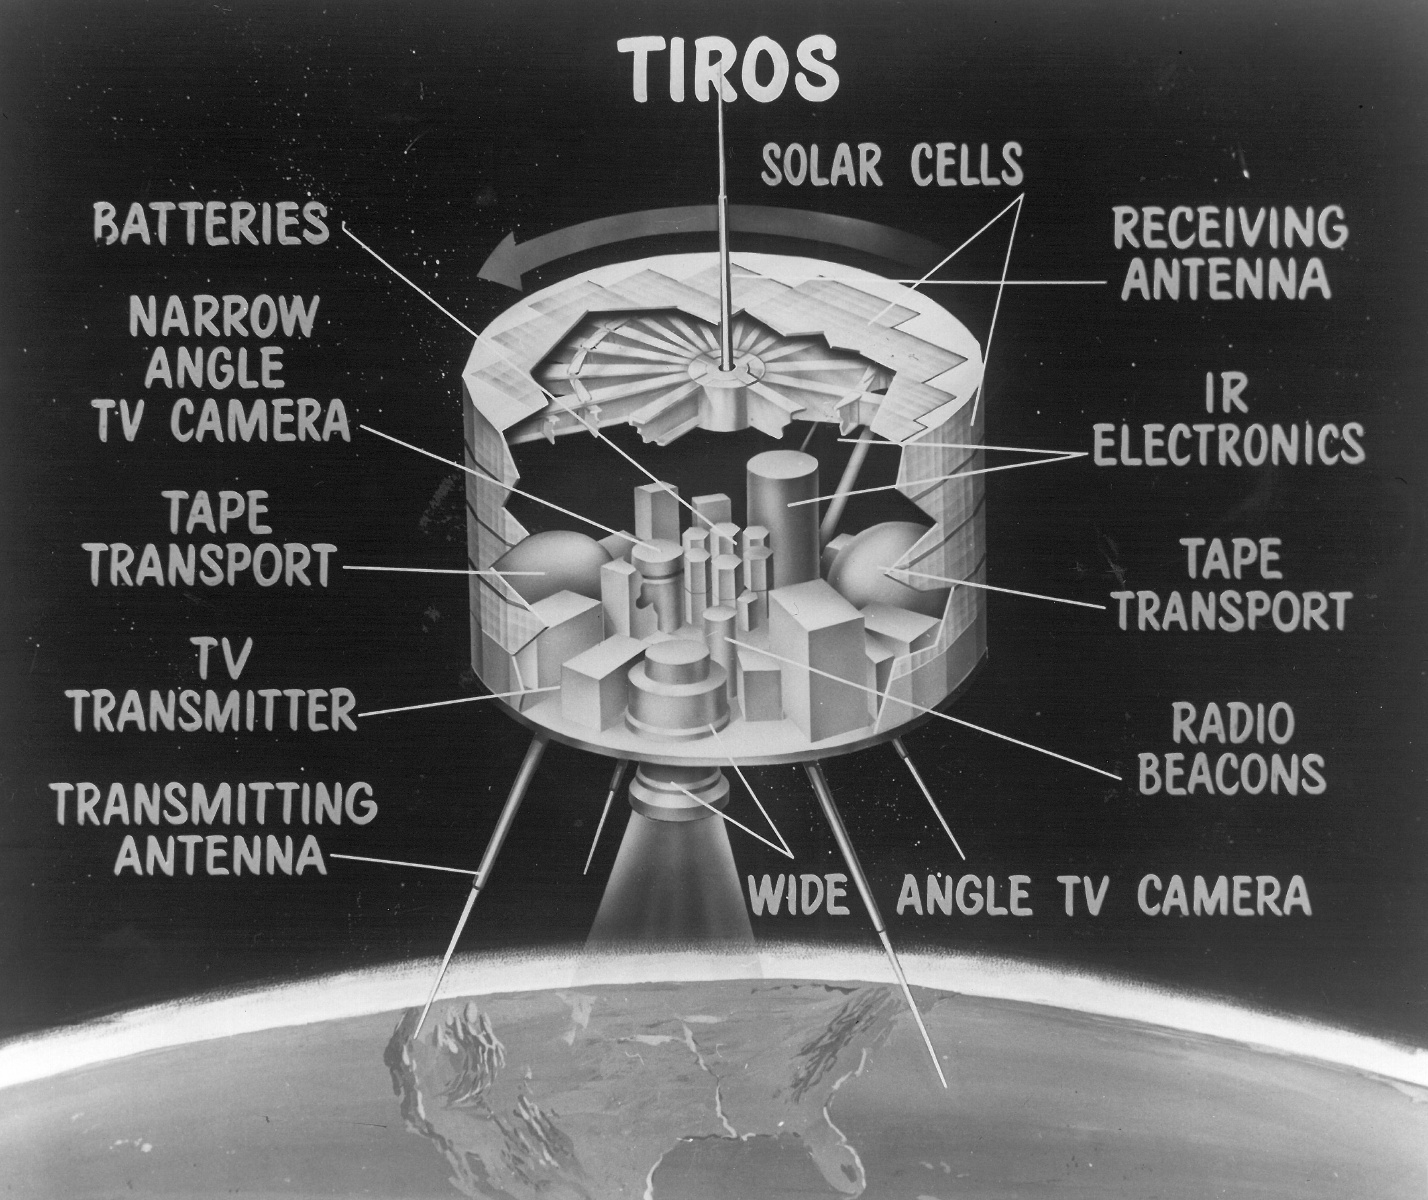
\includegraphics[width=0.65\linewidth]{tiros_1.jpg}
    \caption{A TIROS-1 műhold sematikus felépítése. \url{nesdis.noaa.gov}}\label{tiros}
\end{figure}

A TIROS-1 műholdat további TIROS típusú műholdak (összesen: 10) követték, melyek mind tovább finomítottak a műholdas távérzékelési technológián és az optikai hullámhossz tartományon kívül is méréseket végeztek, pl. infravörös tartomány. A műholdfelvételek elemzői rájöttek, hogy a különböző hullámhossz tartományokban készült felvételekkel nem csak meteorológiai hanem más vizsgálatokat is el lehet végezni. Néhány példát említve: növénytáblák fejlődésének követése és ez alapján termésbecslés, termés-előrejelzés; katasztrófák (erdőtüzek, vulkánkitörések, árvizek) monitorozása, felszínborítottság vizsgálata.\\[15pt]
A képalkotó távérzékelésnek két fő kategóriáját különböztetjük meg:
\begin{itemize}
    \item \textbf{Passzív távérzékelés}: A képalkotás a Napból származó és Földről visszaverődött illetve a Föld termális sugárzásából (IR tartomány) származó elektromágneses hullámok segítségével történik. Csak a nappali áthaladások során használható, kivéve a hőmérsékleti sugárzás hullámhossz tartományában végzett méréseket, melyek a Föld termális sugárzását regisztrálják.
    \item \textbf{Aktív távérzékelés}: A képalkotáshoz szükséges elektromágneses hullámokat a műhold állítja elő és sugározza a Föld felé. Ezen hullámok a Föld felszínéről visszaverődnek és a visszavert hullámok segítségével történik a képalkotás. Előnye, hogy éjszakai áthaladás során is használható, hátránya, hogy megnöveli a képalkotó műszer teljesítményfelvételét.
\end{itemize}

A Föld légkörének transzmisszivitása (a beeső elektromágneses sugárzás energiájának hány százalékát engedi át a légkör) az elektromágneses hullámok esetében csak bizonyos hullámhosszakon 100\%, ezen hullámhossz-tartományokat légköri ablakoknak nevezzük. A műholdas távérzékelésre használt hullámhosszak általában ezen tartományokba esnek.

A \ref{windows}. ábrán a légköri ablakok és műholdas távérzékelésre használt különböző tartományok láthatóak. Eddig csak az optikai tartományról esett szó, ám az ábráról leolvasható, hogy mikrohullámú tartományban is megtalálható egy légköri ablak. A radarral illetve SAR-al felszerelt műholdak a mikrohullámú tartományt használják fel. Mivel mind a Nap, mind a Föld hősugárzásának energiasűrűsége elenyésző a mikrohullámú tartományon, ezért a mikrohullámú érzékelők esetén aktív távérzékelési technikával dolgoznak.

\begin{figure}[H]
    \centering
    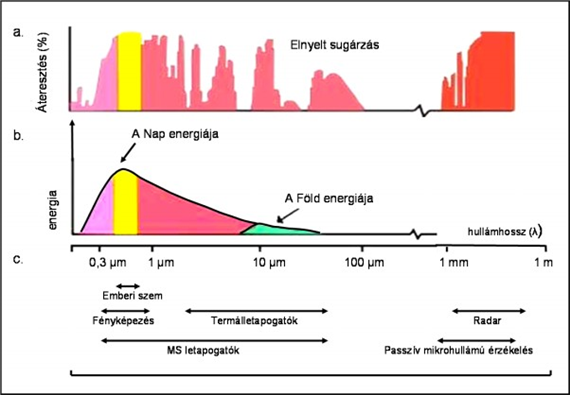
\includegraphics[width=0.75\linewidth]{legkori_ablakok.png}
    \caption{Légköri ablakok: a légkör áteresztőképessége (a), a Nap és a Föld által kibocsájtott elektromágneses energiasűrűség (b) a hullámhossz függvényében és a távérzékelésre használt tipikus hullámhossz-tartományok (c). \url{tankonyvtar.hu}}\label{windows}
\end{figure}

A következő fejezetben bemutatom a SAR technológia alapjait.

\section{Bevezetés a SAR technológiába}

A SAR és InSAR technológiát Bürgmann és társai cikkje \cite{BurgmannInSAR} alapján mutatom be. A technológia részletes leríása megtalálható Ramon Hanssen: \textit{Radar interferometry: data interpretation and error analysis} c. könyvében \cite{RamonHanssen}.

A klasszikus radar (RADAR = RAdio Detection And Ranging) a következő elven működik: a vizsgálandó céltárgyat elektromágneses hullámokkal pásztázzuk és a céltárgyról visszaverődött jel detektálásával és a vett jel feldolgozásával információt szerzünk a céltárgyról. A kétutas futási idő (a hullám kibocsájtásától a vételéig eltelt idő) segítségével a céltárgy távolságát tudjuk megbecsülni és a visszavert jel amplitúdójának segítségével a céltárgy visszaverő-képességére
tudunk következtetni.

A radar térbeli felbontóképességét a radar fizikai mérete, apertúrája limitálja. Ha a távérzékelő műholdak valós apertúrájú radar segítségével készítenének radarképeket a bolygónkról, akkor ezen képek felbontása az $5-\SI{10}{\kilo\meter}$-es tartományba esne. A SAR jelfeldolgozási technikák és pontos műholdpályaadatok felhasználásával jelentősen meg lehet növelni a felszíni felbontást, mely akár a $\SI{10}{\meter}$-t is elérheti \cite{BurgmannInSAR}. Mielőtt a SAR technológia alapjait ismertetném, bevezetek néhány alapfogalmat, melyek segítségével a SAR felvétel készítésének geometriáját jellemzik, melyeket a \ref{ramon:sar_geom}. ábrán is bemutatok.

\begin{figure}[H]
    \centering
    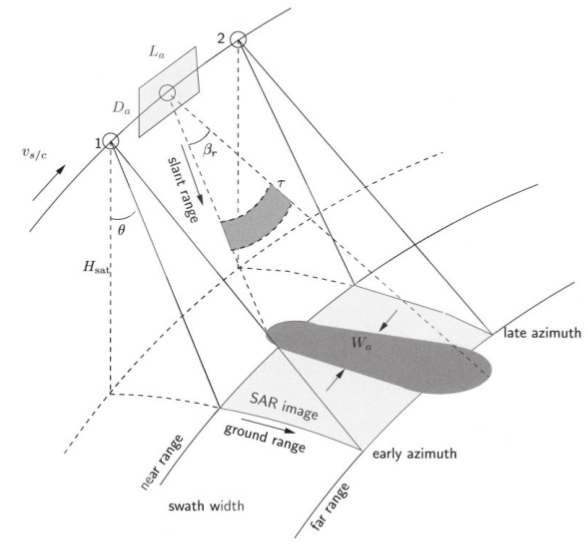
\includegraphics[width=0.75\linewidth]{ramon_SAR.png}
    \caption{SAR felvétel készítésének geometriája. \cite{RamonHanssen}}\label{ramon:sar_geom}
\end{figure}

A \ref{ramon:sar_geom}. ábrán látható SAR alapfogalmak magyarázata \cite{BurgmannInSAR}:
\begin{itemize}
\item azimut (azimuth) irány: a felszínen a műhold haladási irányával megegyező irány,
\item range irány: a felszínen a műhold haladási irányára merőleges irány,
\item pászta szélesség (swath width): egy radar impulzus által megvilágított terület szélessége/kiterjedése.
\end{itemize}

A műholdra helyezett antenna kibocsájtja a mikrohullámokat és regisztrálja a földfelszínről visszaverődött jelet. Egy echó regisztrálásával megközelítőleg a \ref{ramon:sar_geom}. ábrán látható, földfelszíni, sötétszürke színnel jelölt területről kapunk információt. Mivel egy műholdon működő radar folyamatosan mozog a vizsgált tartományhoz képest, ezért a detektált visszavert jeleink Doppler-tolódást szenvednek. A kétutas futási idő, a Doppler-frekvencia tolás és a pontos műholdpálya-adatok segítségével fókuszálni lehet nyers echókat, így nagyobb antenna apertúra ``szintetizálható'' és jelentősen meg lehet növelni a felbontást azimut és range irányban. Egy $100 \times \SI{100}{\kilo\meter}$ szélességű SAR felvétel esetén a tipikus képpont (pixel) mérete: $20 - \SI{100}{\meter}$ \cite{BurgmannInSAR}.

A továbbiakban ismertetem a radar interferometria alapelveit. Bemutatom hogyan lehet a SAR képek fázisinformációját felhasználva felszíni topográfiát és deformációkat vizsgálni.

\section{Az InSAR módszer alapgondolata}

A különböző leképezési eljárások nyers felvételeinek SAR feldolgozásával előálló felvételek az ú.n. SLC (Single Look Complex) felvételek, amelyek egyszeres nézetűek, azaz az átlagolás műveletének alkalmazása nélkül tartalmazzák a felszíni visszaverő cella amplitúdó értékét valamint a két-utas terjedés és az integrált cella fázisérték (felbontási cella objektumainak eredő fázis értéke) eredő fázisát.

A SAR felvétel amplitúdó értéke a földfelszíni felbontási cella elektromágneses valamint geometriai (felszín érdessége, a topográfia meredeksége) tulajdonságaitól függ és egy szürkeárnyalatos képként fogható fel, ahol a világos pixelek a jól reflektáló területek, míg a sötét foltok kevés elektromágneses energiát sugároznak vissza műhold antenna felé.

A jobb és bal oldalról történő visszaverődés okozta kétértelműség elkerülésére a SAR antenna oldalra nézve végzi a felszín leképezését, ezért a radar jelek terjedési útvonala nem merőleges a földfelszínre, illetve a földfelszín topográfiája is igen dinamikus, mely a földfelszínen található egy pixelnek megfelelő felbontási cella különböző módú torzulásához vezethet. Ezen geometriai torzulások a \ref{ramon:shortening}. ábrán láthatóak.

\begin{figure}[H]
    \centering
    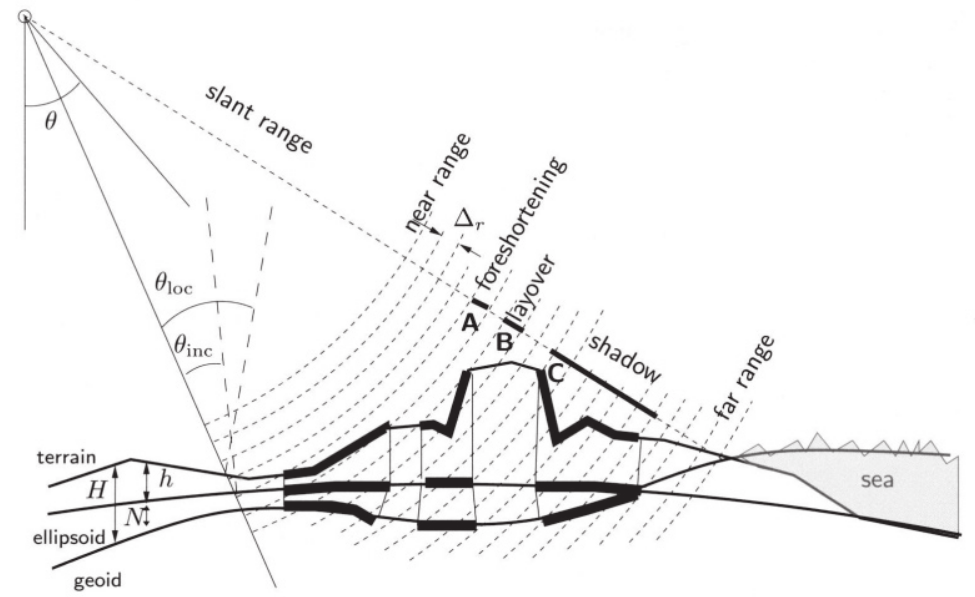
\includegraphics[width=0.75\linewidth]{ramon_shortening.png}
    \caption{A felbontási cella különböző geometriai torzulásokat szenvedhet a topográfia miatt. Pl. \textit{elő-rövidülés} (foreshortening) és \textit{takarás} (layover) esetén a felbontási cellához tartozó terület nagyobb, illetve kisebb lesz. Az is előfordulhat, hogy a topográfia ``leárnyékolja'' egy, vagy több pixelhez tartozó földfelszíni felületet (\textit{shadow}). \cite{RamonHanssen}}\label{ramon:shortening}
\end{figure}

A SAR képek készítésének geometriája miatt a felszálló és leszálló képek más ``nézőpontból'' képzik le a felszínt. Hegyvidékek esetén ez ahhoz vezet, hogy általában a hegy vagy hegyvonulat esetén az egyik oldalt ``megvilágítja'' a radarechó, míg a másik oldal, árnyékban marad. Pl. \ref{merapi}. ábra.

\begin{figure}[H]
    \centering
    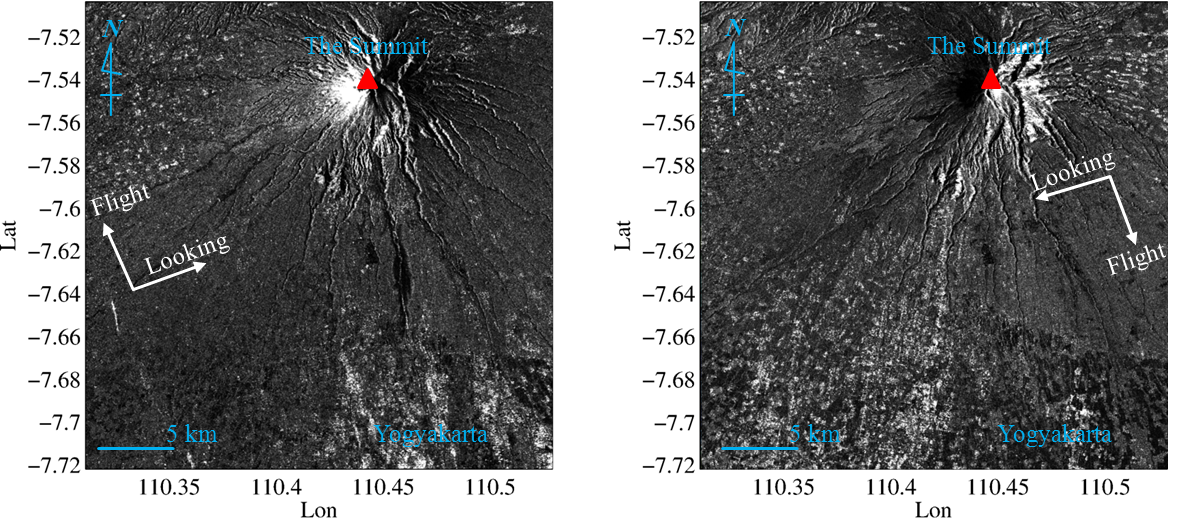
\includegraphics[width=0.8\linewidth]{mt_merapi.png}
    \caption{Bal oldalt felszálló, jobb oldalt leszálló irányból készült SAR felvétel a Merapi-hegyről (Indonézia). Jól látszik, hogy az oldalirányú geometriai leképezés miatt a hegy két oldaláról különböző mennyiségű a visszavert elektromágneses energia. \url{http://asepsaepuloh.com/?m=201401}}\label{merapi}
\end{figure}

Egy SAR kép azonban nem csak a visszavert elektromágneses jel amplitúdóját tartalmazza minden egyes pixel esetén, hanem a fázisát is. Egy képpixel azonban több mikrohullámot visszaverő elemet is tartalmazhat, így egy kép esetén az adott pixel esetén regisztrált fázis a pixelben található összes visszaverő elem fázisválaszának összege, mely véletlenszerűen változik pixelről pixelre.

\subsection{Topográfia leképzése interferometria segítségével}

A fázisinformáció segítségével feltérképezhető egy terület topográfiája vagy két felvétel készítése közben bekövetkezett felszíni deformáció. A módszer elvét az \ref{burgmann:geom}. ábra szemlélteti.

\begin{figure}[H]
    \centering
    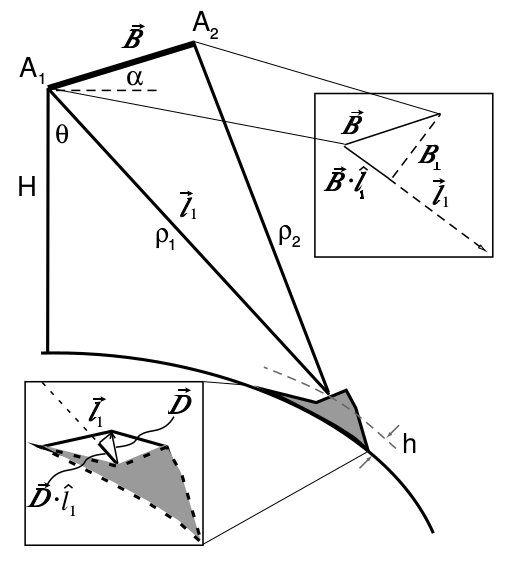
\includegraphics[width=0.5\linewidth]{burgmann_geom.png}
   \caption{Két SAR felvétel készítésének geometriája. A két felvétel fáziskülönbsége több tagból adódik: a felvételi pozíciók (náhány száz méteres) eltéréséből ($\vec{B} \ne 0$) és a felszíni deformációból ($\vec{D}$) \cite{BurgmannInSAR}}\label{burgmann:geom}
\end{figure}

A \ref{burgmann:geom}. ábrán $A_1$ és $A_2$ jelöli a műholdpozíciókat a felvételek készítésének időpontjában, $\vec{B}$ az $A_1$-ből az $A_2$-be mutató bázisvonal vektor, $\vec{l}_1$ a műhold-pixel irány vagy látóirány (line-of-sight, LOS) az $A_1$ felvétel esetén, a $H$ egy adott referencia felszínhez képest mért repülési magasság, $\rho_1$ és $\rho_2$ a vizsgált pixel pont távolsága $A_1$ és $A_2$ pozíciótól, $\vec{D}$ az $A_1$ és $A_2$ felvételek készítésének időpontjai között eltelt idő alatt bekövetkezett deformáció. A bázisvonal vektor két komponensre bontható: egy $\vec{l}_1$-el párhuzamos $B_{\parallel}$ és egy $\vec{l}_1$-re merőleges $B_{\perp}$ komponensre.

A felszíni topográfia és deformáció vizsgálata a két kép fáziskülönbségeinek felhasználásával történik. A fáziskülönbségek kiszámítása előtt el kell végezni a képek koregisztrációját. Mivel két kép készítésének geometriája nem azonos (különböző térbeli pozícióból készült a két felvétel) ezért egyazon felszíni visszaverőpont képi koordinátája nem azonos a két esetén. Ezért a fáziskülönbségek kiszámítása előtt (interferogram készítése) az egyik képet kiválasztjuk ún. mesterképnek és egy algoritmus segítségével kiszámítjuk azt a transzformációt, mely az ún. szolga képet a mesterképhez regisztrálja.

A koregisztráció után elkészíthető az interferogram. A fáziskülönbség értékét egy pixel esetén jelölje $\Phi$. Most tegyük fel, hogy a két felvétel készítése közötti eltelt időben semmilyen változás nem következett be az atmoszférában és felszíni deformáció sem történt. Ha egy adott pixel esetén a visszaverő elemek fázisválasza nem változik, akkor a fáziskülönbsége egy adott pixel esetén ($\Phi$) kizárólag a $\rho_1$ és $\rho_2$ távolságoktól függ \cite{BurgmannInSAR}:
\begin{equation}\label{topo_phase}
    \Phi = \frac{4 \pi}{\lambda} (\rho_2 - \rho_1)
\end{equation}
A $B \ll \rho_{1,2}$ közelítést alkalmazva (párhuzamos sugárút közelítés) a következő egyenlethez jutunk \cite{ZebkerGoldstein1986}:
\begin{equation}\label{los_par}
    \Phi \approx - \frac{4 \pi}{\lambda} (\vec{B} \cdot \vec{l}_1 ).
\end{equation}
Az egyenlet szerint a fázis arányos a bázisvonal vektor $\vec{l}_1$ LOS irányra vetített komponensével, $B$-vel. Figyelembe véve a felvételek készítésének geometriáját megkaphatjuk egy adott pixel ponthoz tartozó $h = H - \rho_1 \cos\theta$ referencia felülettől mért magasságot, ha a (\ref{los_par}) egyenletből kifejezzük a $\theta$ értékét \cite{BurgmannInSAR}:
\begin{equation}\label{theta_phi}
    \theta = \arcsin \left(-\frac{\lambda\Phi}{4 \pi B}\right) + \alpha.
\end{equation}

\subsection{Fáziskicsomagolás}

Mivel a fázis $2\pi$-ként periodikus, ezért egy adott pixel fázisa a következőképpen írható fel: $\Phi + n \cdot 2\pi$, ahol $n \in \mathbb{N}$. A fáziskicsomagolás (\textit{unwrapping}) lépése a két szomszédos pixel között jelentkező $\Delta n = 1$ vagy $\Delta n = -1$ értékének meghatározása. A kicsomagolás bemenő fázisértékeit nevezik becsomagolt fázisnak (\textit{wrapped}) és a kimenő értékeket pedig kicsomagolt fázisnak (\textit{unwrapped}). A kicsomagolt fázisértékeket a (\ref{theta_phi}) egyenletbe visszahelyettesítve, megkaphatóak a felszín feletti magasságértékek. A kicsomagolt és becsomagolt fázis közötti különbségek a \ref{unwrapping} ábrán láthatóak.

\begin{figure}[H]
    \centering
    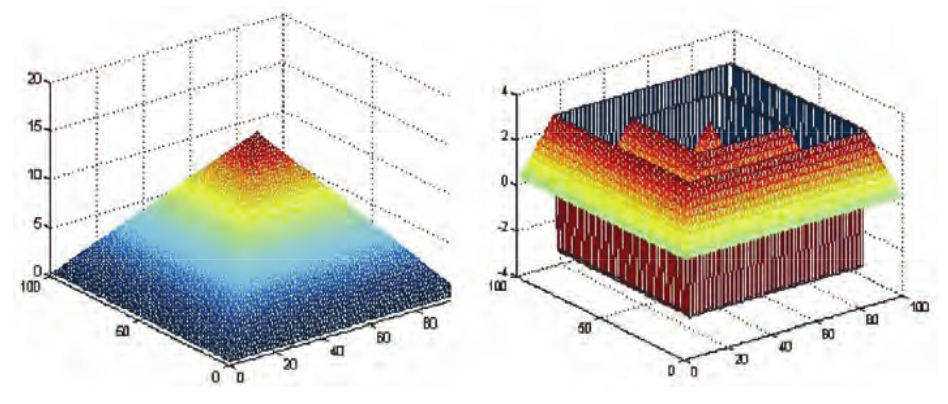
\includegraphics[width=0.6\linewidth]{esa_phase_unwrap.png}
    \caption{Fáziskicsomagolást bemutató ábra. Bal oldalon kicsomagolt-, jobb oldalon a becsomagolt fázis látható. A fáziskicsomagolás során a jobboldali ábrán látható fázisugrásokat szüntetjük meg. (InSAR Principles: Guidlines for SAR Interferomatry Processing and Iterpretation (ESA TM-19)}\label{unwrapping}
\end{figure}

Fontos megjegyezni, hogy az interferogram készítést számos előfeldolgozási lépés előz meg. Az előfeldolgozás indulhat a nyers SAR kép adatokból, illetve az ún. Single-Look Complex (SLC) képekből. Jelen dolgozat elkészítésénél használt előfeldolgozási lépéseket és a feldolgozáshoz használt programokat a (\ref{programs}) fejezetben ismertetem.

Az SRTM (Shuttle Radio Topography Mission) digitális magassági modell \cite{SRTM} is ennek a technológiának köszönheti a létrejöttét. A misszió során az Endeavour űrsiklóra szerelt kettő darab radarantenna segítségével végeztek el méréseket, melyek interferometrikus feldolgozásával származtatták az első globális magassági modellt.

Egy a topográfiai fázist bemutató interferogram látható a \ref{insar_topo}. ábrán.

\begin{center}
    \begin{figure}[H]
        \centering
        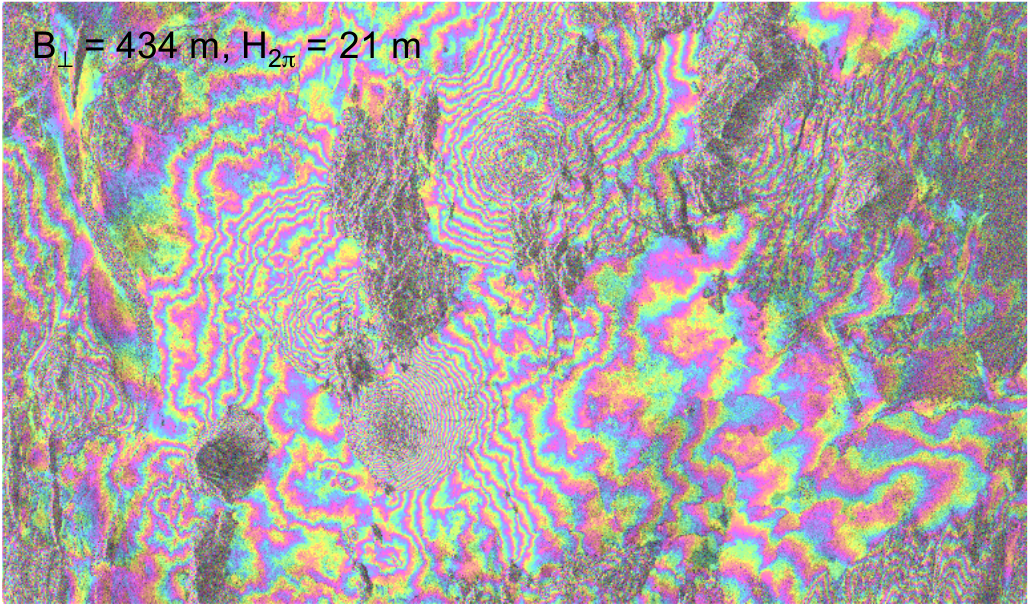
\includegraphics[width=0.75\linewidth]{hooper_topo_2.png}
        \caption{Topográfiai fázist tartalmazó interferogram. Háttérben a SAR amplitudó kép látható. A színskála a becsomagolt fázisértékeket mutatja. A képen látható mintázat a korábban említett $2\pi$ szerinti periodicitás eredménye. Egy térbeli tartományt, ahol a fázisértékek $0$-tól $2\pi$-ig növekednek interferencia csíknak (\textit{fringe}-nek) nevezünk. Egy interferencia csík adott szintemelkedésnek felel meg, mely függ a merőleges bázisvonaltól. Jelen esetben egy interferencia csík $\SI{21}{\meter}$-es szintemelkedésnek felel meg. \cite{HooperThesis}}\label{insar_topo}
    \end{figure}
\end{center}

\subsection{Felszíni deformációk feltérképezése interferometria segítségével}

Az eddigi számítások során feltételeztük, hogy nem történt felszíni deformáció. Most megvizsgáljuk azt az esetet, mikor a két felvétel készítése között eltelt időben felszíni deformáció történt. Ebben az esetben az (\ref{los_par}) egyenletben megjelenik egy plusz deformációs tag \cite{BurgmannInSAR}:
\begin{equation}\label{los_par_def}
    \Phi \approx \frac{4 \pi}{\lambda} (-(\vec{B} \cdot \vec{l}_1 ) + (\vec{D} \cdot \vec{l}_1)).
\end{equation}
Ahogyan korábban most, is feltételeztük, hogy a bázisvonal vektor sokkal kisebb mint a $\rho_{1,2}$ távolság, illetve, hogy ez igaz a deformációs vektorra is. Ahhoz, hogy megkapjuk a deformációs tagot először a topográfia által okozott fázist kell eltávolítani az egyenletből. Ez megtehető DEM (Digital Elevation Model - Digitális Domborzati Modell) magasságértékekkel és pontos pályaadatokkal elvégzett korrekcióval. A 2000-es évek előtt, mikor még nem állt rendelkezésre pontos, jó felbontású globális DEM, három felvételre volt szükség a deformáció vizsgálatához. Két felvétel segítségével készítették el a topográfiai tag eltávolításához szükséges DEM-et és a harmadik felvételt egy másikkal összepárosítva vizsgálták a felszíni deformációkat. Az (\ref{los_par_def}) egyenlet alapján látható, hogy kizárólag LOS irányú deformációk detektálása lehetséges az InSAR módszerrel. Természetesen ahhoz, hogy a LOS irányba történt felszíni deformáció értékeit meghatározhassuk, a fázist ki kell csomagolni.

Egy példa interferogram látható a \ref{izmit}. ábrán. Az interferogram egy Izmitben (Törökország) történt földrengés okozta deformációs fázistagot mutatja be.

\begin{figure}[H]
    \centering
    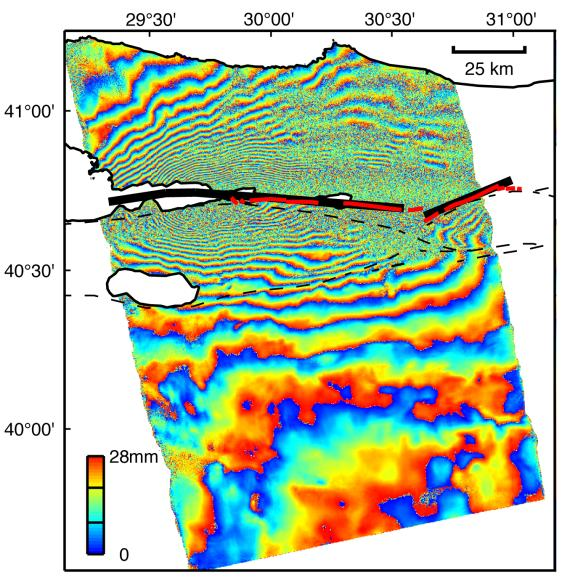
\includegraphics[width=0.5\linewidth]{izmit_interferogram.jpg}
    \caption{Az izmiti (Törökország) földrengés interferogramja a becsomagolt fázissal. A földrengés előtt és után készült felvételekből előállított interferogramon a földrengés okozta LOS irányú elmozdulások láthatóak. A fekete vonalak a szeizmikus törésvonalakat jelölik. (NASA/JPL-Caltech)}\label{izmit}
\end{figure}

A SAR képek fázisinformációját felhasználva az InSAR módszer segítségével lehetséges mind a topográfia, mind a felszíni deformációk térbeli vizsgálata. Felszíni deformációk  vizsgálatánál, egyetlen interferogram felhasználásával csak a két felvétel között eltelt időben bekövetkezett deformáció vizsgálható. Ha azonban a felszíni deformációs folyamatokat időben szeretnénk vizsgálni, akkor több felvételre van szükségünk, melyek lefedik a számunkra érdekes időintervallumot. Egyetlen interferogram nagy erejű földrengések okozta deformációk tanulmányozására ideális, mivel földrengések esetén a releváns információ felszíni elmozdulások mértéke, melyeket a földrengés kipattanása okozott, ``egyetlen'' időpillanatban.

Fontos megjegyezni, hogy nem minden képpár esetén kapunk azonos ``minőségű'' interferogramot. A következő fejezetben bemutatom az időbeli és térbeli szeparáció növekedése miatt megjelenő dekorrelációt, azaz a koherencia csökkenésének folyamatát.

\subsection{Időbeli és térbeli dekorreláció}

Két felvétel közötti, statisztikai értelemben vett, hasonlóságot a koherenciával (korrelációval), jellemezhetjük, melyet a következőképpen számíthatunk ki \cite{BurgmannInSAR}:
\[
    \gamma = \frac{|\langle s_1 s_2^* \rangle|}{\sqrt{\langle s_1 s_1^*
    \rangle \langle s_2 s_2^* \rangle}},
\]
ahol $s_1$ és $s_2$ a két felvétel komplex pixelértékei (amplitúdó és fázis), $\langle \cdot \rangle$ jelöli a pixelértékekre végzett átlagolást és $s^*$ az $s$ komplex szám komplex konjugáltja. $\gamma = 1$, ha a két felvétel megegyezik és $0$, ha teljesen különböznek. A gyakorlatban az átlagolást nem az egész képre végzik el, hanem egy mozgó ablakkal számítják ki a képen található különböző területekre.

Egy interferogram esetén a teljes koherencia a legtöbb esetben négy tagból tevődik össze \cite{HooperThesis}:
\[
    \gamma = \gamma_{\text{időbeli}} \cdot \gamma_{\text{térbeli}} \cdot \gamma_{\text{doppler}} \cdot \gamma_{\text{termális}}.
\]

Az egyes tagokat egy egyszerű modell segítségével becsülhetjük meg \cite{HooperThesis}:
\begin{align}
    \gamma &= \gamma_{\text{időbeli}} \cdot \gamma_{\text{térbeli}} \cdot \gamma_{\text{doppler}} \cdot \gamma_{\text{termális}},\\
    &= \left(1 - f \left(\frac{T}{T^c}\right)\right) \left(1 - f \left(\frac{B_{\perp}}{B^c_{\perp}}\right)\right) \left(1 - f \left(\frac{F_{\text{DC}}}{F^c_{\text{DC}}}\right)\right) \gamma_{\text{termális}}. \label{stack_model}
\end{align}
ahol,
[\
    f(x) = \begin{cases*}
            x, & ha $x \le 1$\\
            1, & ha $x \ge 1,$
            \end{cases*}
\]
$T$ jelöli az időbeli bázisvonalat, $B_{\perp}$ pedig a térbeli merőleges bázisvonal komponensét. $F_{\text{DC}}$ a Doppler-centriod értéke. A $c$ index a különböző paraméterek kritikus értékét jelöli. A kritikus paramétereket általában függnek a vizsgált felszín típusától (száraz sivatagos a vizsgált terület vagy növénnyel borított) és a műholdra felhelyezett SAR műszertől is. ERS műhold adatok esetén, ha száraz területről készül felvételeket vizsgálunk a tipikusan használt értékek: $T^c = 5\text{ év}$, $B^c_{\perp} = \SI{1100}{\meter}$ és $F^c_{\text{DC}} = \SI{1380}{\hertz}$ \cite{HooperThesis}.

Az időbeli dekorrelációt az okozza, hogy a a visszaverő felszín változik az idő elteltével. A vegetáció erősen megnöveli az időbeli dekorreláció mértékét, mivel a növényeken található szórópontok visszaverő tulajdonságai idővel változnak. Egy másik fontos tényező az atmoszféra állapotának változása két felvétel között, amely a radarhullámok terjedési útjának és sebességének a változását okozza. Ha az elektromágneses hullám terjedési sebessége a hullám terjedési út mentén megváltozik, egy előző állapothoz képest, megváltozik a kétutas futási idő és ezáltal a detektált fázisérték is. További dekorrelációs források az évszakos hatások, mint pl. a hótakaró megjelenése.

A termális korrelációs tag becslésere a következő kapcsolat áll rendelkezésünkre:
\[
    \gamma_{\text{termális}} = \frac{1}{1 + \text{SNR}^{-1}},
\]
ahol SNR a visszavert radarhullám jel-zaj aránya (Signal to Noise Ratio). Általános esetben, amikor a korreláció értékét kívánjuk kiszámítani, a termális tag értékét vagy konstansnak vagy nagy SNR-t feltételezve 1-nek veszik.

Több interferogram esetén becsülhető az ún. \textit{stack}-koherencia, az egész adatrendszerre vonatkozó koherencia érték, mely az egyes interferogramok koherencia értékeinek összege, azaz $\gamma_{\text{stack}} = \sum_{i=1}^{N} \gamma_{\text{teljes}, i}$. A gyakorlatban a (\ref{stack_model}.) egyenlet használják fel az egyes interferogramok koherencia tagjainak becslésére, a termális koherencia tagot állandónak. A mesterképet úgy érdemes kiválasztani, hogy az a stack-koherenciát maximalizálja.

Ahhoz, hogy a felszíni deformációt pontosan tudjuk meghatározni, olyan interfereogramokra van szükségünk, melyek koherensek, azaz pixeleiknek nagy része koherens maradt az összes interferogramon. Az atmoszféra állapotának változása, a vegetáció jelenléte, a nagy időbeli és térbeli bázisvonalak lerontják a koherenciát, dekorrelációt okoznak, ezért törekedni kell arra, hogy olyan képpárokból készítsünk interferogramokat, melyek kis bázisvonalakkal rendelkeznek.

A fentiekben leírtak következménye, hogy az InSAR módszer nem vegetált, kopár, sziklás illetve városi környezet vizsgálatára a legalkalmasabb. A különböző hatások miatti dekorreláció megnehezíti és bizonyos esetekben ellehetetleníti a deformációs jel visszaállítását. Az interferogramok elkészítésénél törekedni kell a koherencia megőrzésére. Erősen vegetált régió vizsgálatánál számítani kell arra, hogy az interferogramok kis- vagy nagyrészt inkoherensek lesznek és emiatt a koherens szórópontok nem fogják egyenletesen lefedni a vizsgált területet, térbeli eloszlásuk inhomogén lesz.

A következő fejezetben a több interferogram segítségével végzett idősorelemzést mutatom be.

\section{Idősorelemzés több interferogram felhasználásával}

Az előző fejezetekben megvizsgáltuk, hogy idealizált esetben (atmoszféra és egyéb zajtényezők hatása elhanyagolható, a fáziskülönbséget a terjedési úthosszak különbsége és a deformáció okozza) egyetlen interferogram esetén, a pixelek fáziskülönbség értéke, mely fázistagokból adódik. Ha több SAR felvétel áll rendelkezésünkre, akkor lehetségessé válik több interferogram elkészítésével a felszíni deformációk időbeli vizsgálata. Mivel a radarinterferometria relatív technika, azaz a két felvétel pixeljeinek abszolút térbeli helyzetét nem, csak a pixelek térbeli helyzetének változását képes detektálni, ezért az idősorelemzés elején ki kell választani egy mesterképet, melyhez képest vizsgáljuk a felszíni elmozdulásokat.

Ahogy korábban már említettem, egy pixelen belül több szórópont fázisválaszából adódik össze a pixel fázisértéke. Ez alapján több fő esetet különböztetünk meg, melyeket a \ref{scatterer_types}. ábrán is bemutatok:

\begin{figure}[H]
    \centering
    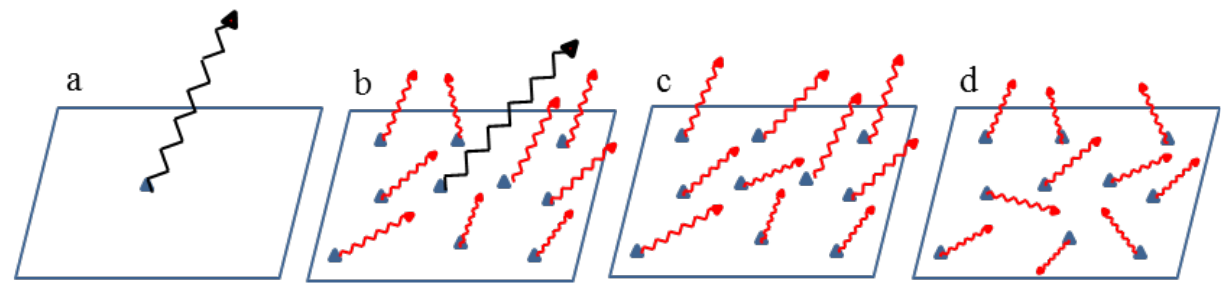
\includegraphics[width=0.85\linewidth]{scatterers.png}
    \caption{Különböző szórópontokkal rendelkező pixelek: (a) egyetlen szórópontot tartalmazó pixel, (b) domináns és elosztott szórópontokat tartalmazó pixel, (c) elosztott szórópontokat tartalmazó koherens pixel, (d) elosztott szórópontokat tartalmazó inkoherens pixel. \cite{Banyai2014}}\label{scatterer_types}
\end{figure}

\begin{enumerate}[(a)]
    \item a pixelben egyetlenegy szórópont van, mely egyedül határozza meg a pixel fázisértékét,
    \item a pixelen belül több szórópont van, melyek közül egy domináns szórópont fázisa jóval nagyobb súllyal adódik a pixel fázisértékéhez, mint a többi szóróponté,
    \item a pixel fázisértéke több szórópont fázisából áll össze, összegük még koherens pixelt eredményez,
    \item a pixel fázisértéke több szórópont fázisából áll össze, véletlen szerű fázisösszeget, inkoherens pixelt eredményez.
\end{enumerate}

Az interferogramok pixeljeinek feldolgozására több módszert is kifejlesztettek. \cite{Ferretti2011, Hooper2008, Ferretti2001, Lanari2002} A feldolgozási módszerek két fő irányzatot követnek:

Az első módszer, a \textbf{Permanens Szórópontú Interferometria} (PSI - Permanent Scatterer Interferometry). A módszer lényege, hogy, olyan pixeleket használ fel az idősorelemzéshez és a felszíni deformációk meghatározásához, melyek fázisa ``stabil'' marad a különböző interferogramok esetében. Ezek tipikusan a domináns szóróponttal rendelkező pixelek. A fázisstabilitás ``mérése'' nem triviális probléma, több módszert is kidolgoztak a mértékének a meghatározására \cite{Ferretti2001, Hooper2008}.

A PSI elemzés során igen nagy időbeli és térbeli bázisvonalakkal terhelt interferogramok is keletkezhetnek. Mivel az idősorelemzés során felhasznált képek több éves időszakot is lefedhetnek a mesterkép és szolgaképek fáziskülönbségeit tartalmazó interferogramok, időbeli bázisvonalai több évesre nőhetnek fel, mely nagyfokú időbeli dekorrelációhoz vezethet. Hasonlóan a térbeli bázisvonalak hossza is nagy lehet, mely további térbeli dekorrelációt okoz.\\[15pt]
A második feldolgozási eljárás az ún. \textbf{rövid bázisvonalú}, \textbf{SBAS} - Small BAseline Subset módszer, amelyet olyan pixelek feldolgozására fejlesztették ki, melyek elosztott szóróponttal rendelkeznek \cite{Ferretti2011} (DS - Distributed Scatterers, \ref{scatterer_types}. ábra (c) pixeltípus). A módszer előnye, hogy rövid idő- és térbeli bázisvonalú interferogramokból állít elő egy hálózatot, ezzel biztosítva a koherencia megmaradását egy-egy felvétel között. Ha rendelkezünk megfelelően kicsi bázisvonalú interferogramokkal, akkor redundanciát beépítve a hálózatba a kicsomagolt fázisértékek ellenőrzésére is lehetőségünk nyílik. A két módszer közötti különbséget a \ref{psi_sbas}. ábra mutatja be.

A szakdolgozat elkészítése során a Hooper és társai \cite{Hooper2008, Hooper2012} által kifejlesztett \stamps (Stanford Method for Persistent Scatterers)  programot használtam fel. A program az interferogramok feldolgozása során megkeresi a PS pixeleket és segítségükkel elvégzi a fáziskicsomagolást és a deformációk idősorelemzését. A program hullámszám- és frekvencia szerinti szűrést, Goldstein-szűrést \cite{GoldsteinFilter} alkalmaz a jel-zaj arány növelésére és a PS pixelek kiválasztására. A technika előnye, hogy olyan területeken is lehetővé teszi az interferometrikus vizsgálatok elvégzését, ahol egyébként a terepviszonyok miatt ez nem lenne lehetséges (pl. vegetációval borított területek), illetve nem szükséges \textit{a priori} modell a deformációk meghatározásához, tehát tetszőleges időbeli lefolyással rendelkező deformáció vizsgálható a program segítségével. A \stamps további előnye, hogy az módszer SBAS módszerrel elkészített interferogramokat is képes feldolgozni \cite{Hooper2008}, illetve, hogy a PSI és SBAS módszerrel elvégzett idősorelemzés során kapott adatrendszert képes egyesíteni. Hátránya, hogy a program kezelésének elsajátítása hosszabb időt igényel, a feldolgozás összetettsége miatt (különböző szűrők alkalmazása) hosszabb ideig tart a feldolgozás és sokszor a felhasználónak kell megkeresnie az optimális feldolgozási paramétereket. A \stamps programról bővebben a \ref{stamps} fejezetben lehet olvasni.

\begin{figure}[H]
    \centering
    \includegraphics[width=0.8\linewidth]{psi_vs_sbas.png}
    \caption{PSI és SBAS interferogramok hálózata. A fekete körök jelölik a SAR felvételeket, a folytonos vonalak a két kép között készült interferogramot. $B_{\perp}$ jelöli a merőleges bázisvonal értékét.}\label{psi_sbas}
\end{figure}

A fentiekben bemutatott műholdradar interferometriára épülő, idősorlemző eljárásokat szokás Multi-Temporal InSAR-nak, MTInSAR-nak nevezni.

Ha a felszálló (ASC) és leszálló (DSC) irányból készült felvételeket külön-külön InSAR idősorelemzéssel feldolgozzuk, akkor két sebességmezőt kapunk. A két sebességmező eltérő LOS irányban adja meg a sebességértékeket. A sebességmezők kombinálásával becsülhetőek a vertikális és kelet-nyugati sebességkomponensek, feltéve, hogy elegendő ASC és DSC adatpont áll rendelkezésre. A \ref{daisy} fejezetben ismertetem a Geodéziai és Geofizikai Intézetben kifejlesztett DAISY programrendszert, mely az ASC és DSC LOS sebességek kombinálásával becsli meg a  fent említett sebességkomponenseket.

\section{A \stamps idősorelemzés}\label{stamps}

A \stamps program a \texttt{Matlab} környezetre alapul, a \stamps feldolgozás rutinjai \texttt{Matlab} nyelven íródtak. A nyers SAR felvételek fókuszálása a \texttt{ROI\_PAC} programmal történik, az interferogramok elkészítését és a topográfiai tag eltávolítását a \texttt{DORIS} programcsomag végzi, \texttt{unix} környezetben. Az előfeldolgozás után az egyes interferogram pixelek fázisértéke a következőképpen írható fel \cite{HooperThesis}:
\begin{equation}\label{stamps_phase}
    \Delta\Phi = \Phi_{\text{def}} + \Delta\Phi_{\text{DEM}} + \Delta\Phi_{\text{atmo}} + \Delta\Phi_{\text{pálya}} + \Phi_{\text{zaj}},
\end{equation}
ahol
\begin{itemize}
    \item $\Delta\Phi$: a fáziskülönbség egy interferogram pixel esetén,
    \item $\Phi_{\text{def}}$: a deformáció okozta fáziskülönbség,
    \item $\Delta\Phi_{\text{DEM}}$: a topográfiai tag eltávolításához használt DEM hibájából adódó fázistag,
    \item $\Delta\Phi_{\text{atmo}}$: az atmoszféra állapotának megváltozásából származó fáziskülönbség, atmoszferikus hatás (APS - atmospheric phase screen),
    \item $\Delta\Phi_{\text{pálya}}$: műholdpályaadatok hibájából származó fázistag,
    \item $\Phi_{\text{zaj}}$: egyéb zajtényező.
\end{itemize}
A (\ref{stamps_phase}) egyenletben található tagok változó térbeli és időbeli korrelációval rendelkeznek, melyeket a \ref{phase_corr}. táblázat foglal össze.

\begin{table}[H]
    \centering
    \begin{tabular}{l l l} \toprule
        Fázistag & térbeli jellemző & időbeli jellemző\\ \midrule
        $\Phi_{\text{def}}$ & hosszú hullámhosszú & alacsony frekvenciájú\\
        $\Delta\Phi_{\text{DEM}}$ & hosszú hullámhosszú & bázisvonallal korrelált \\
        $\Delta\Phi_{\text{atmo}}$ & hosszú hullámhosszú & magas frekvenciájú\\
        $\Delta\Phi_{\text{pálya}}$ & hosszú hullámhosszú & magas frekvenciájú \\
        $\Phi_{\text{zaj}}$ & rövid hullámhosszú & magas frekvenciájú \\ \bottomrule
    \end{tabular}
    \caption{$\Delta\Phi$ interferometrikus fázis tagjainak tér- és időbeli jellemzői. \cite{Hooper2012}}\label{phase_corr}
\end{table}

A \ref{phase_corr}. táblázatban jellemzett tulajdonságokat kihasználva megbecsülhető a a felbontási cella fáziszaj értéke. A deformáció fázis mind térben, mind időben korrelált (hosszú hullámhosszú); ezzel szemben az atmoszferikus fázis csak térben korrelált, időben az egyes interferogramok gyorsan változó atmoszferikus hatással terheltek (nagy frekvencia). A műholdpályahiba egy-egy interferogramon hosszú hullámhosszú fázis tagként jelentkezik, azonban interferogramról interferogramra változik. A DEM hiba okozta fázis tag is hasonló tér-és időbeli tulajdonságokat mutat, ezen kívül a DEM hiba okozta fázis egy része korrelál a merőleges bázisvonal értékével. A térben korrelált $\Delta\Phi^{\text{tk}}$ tagot, mely nemcsak a $\Phi_{\text{def}}$, $\Delta\Phi_{\text{atmo}}$ és $\Delta\Phi_{\text{pálya}}$ tagok becsült értékét, hanem a $\Delta\Phi_{\text{DEM}}$ és $\Phi_{\text{zaj}}$ térben korrelált részét is tartalmazza, eltávolítva a (\ref{stamps_phase}) egyenletből a következő összefüggéshez jutunk:
\begin{equation}\label{phase_noncorr}
    \Delta\Phi - \Delta\Phi^{\text{tk}} = \Delta\Phi_{\text{DEM}}^{\text{tnk}} + \Phi_{\text{zaj}}^{\text{tnk}},
\end{equation}
ahol $\Delta\Phi_{\text{DEM}}^{\text{tnk}}$ és $\Phi_{\text{zaj}}^{\text{tnk}}$ a DEM hiba- és zaj fázistag térben nem korrelált összetevője. A \stamps a térben korrelált tagot Butterworth- és adaptív szűrők segítségével határozza meg. A $\Delta\Phi_{\text{DEM}}$ DEM hiba fázistag arányos a merőleges bázisvonallal ($\Delta\Phi_{\text{DEM}} = B_{\perp} K$, $K$ arányossági tényező), így legkisebb négyzetes módszerrel becsülhető és eltávolítható \ref{phase_noncorr} egyenletből, meghagyva a zaj fázistag térben nem korrelált részét. A megmaradt fázistag segítségével definiálható egy pixel időbeli koherenciája (temporal coherence), melynek segítségével jellemezhető egy pixel fázisának stabilitása:
\begin{equation}\label{temp_coh}
    \gamma_x = \frac{1}{N} \left| \sum_{i=1}^{N} \exp \left\{ j \left(\Delta\Phi_{x,i} - \Delta\Phi_{x,i}^{\text{tk}} - \Delta\Phi_{\text{DEM}, x,i}^{\text{tnk}} \right) \right\} \right|
\end{equation}
ahol $i = 1,..,N$ az $N$ db interferogramot indexeli, $x$ pedig az interferogramok pixeleit és $j = \sqrt{-1}$. $\gamma_x = 1$ a zajmentes pixel esetén és $\gamma_x = 0$ a véletlenszerű fázissal rendelkező pixel esetén. A PS-ek kiválasztása valószínűségi alapon zajlik:
\begin{enumerate}
    \item $\gamma_x$ kiszámítása interferogramokra és generált véletlen fázissal rendelkező adatrendszerre.
    \item A két $\gamma_x$ adatrendszerből ki lehet számítani $\gamma_x$ hisztogramját H($\gamma_x$).
    \item Feltételezés: $\gamma_x$ < 0.3 értékkel rendelkező pixelek nem PS pixelek, azaz\\H($\gamma_x$ < 0.3) = 0. Ezen összefüggés felhasználásával lehet a H($\gamma_x$) függvényt normalizálni és megkapni a PDF($\gamma_x$) függvényt, azaz a $\gamma_x$ valószínűségi sűrűségfüggvényét.
    \item A PDF($\gamma_x$) alapján lehet a PS pixeleket kiválogatni. Ennél a lépésnél a felhasználónak meg kell adnia, hogy milyen arányban kerüljenek a PS pixelek közé nem-PS pixelek.
\end{enumerate}
A probléma az, hogy a $\gamma_x$ értékek kiszámítása előtt ismerni kell a magukat a PS pixeleket, tehát szükség van ``előzetes'' PS pixelekre, melyek segítségével elvégezhető a $\gamma_x$ kiszámítása és kijelölhetőek az új PS pixelek, majd ezt a lépést iterálva végül eljutunk a valós PS pixelekig. Az előzetes pixeleket a \cite{Ferretti2001} által definiált amplitúdó diszperziós index alapján választja ki a program. Az amplitúdó diszperzió definíciója:
\[
    D_{\text{A}} = \frac{\sigma_{\text{A}}}{\mu_{\text{A}}}.
\]
Egy pixel esetén a pixel amplitúdó idősort vizsgálva $\sigma_{\text{A}}$ az idősorban szereplő amplitúdó értékek szórása, $\mu_{\text{A}}$ pedig az idősor értékek átlaga. A program azon pixeleket választja ki előzetes PS-nek, melyek $D_{\text{A}}$ értéke kisebb egy felhasználó által megadott értéknél. Ezt az értéket 0.4-nek szokták megválasztani PSI elemzésnél.

SBAS feldolgozás esetén a \stamps nem amplitúdó diszperziós indexet használja fel az előzetes szórópontok kijelölésére, hanem az amplitúdó különbségek szórását, melyet úgy számít ki, hogy minden interferogram esetén a fázis- és amplitúdó különbségeket is kiszámítja és az amplitúdó különbségek értékeinek szórása alapján válogatja ki az előzetes szórópontokat.

A PS pixelek kiválasztásánál a \stamps a véletlenszerű fázissal rendelkező pixelek felszíni sűrűségét ($\text{nem-PS pixel}/\text{km}^2$) is meghatározza, a $\gamma_x$ valószínűségi sűrűség függvény alapján. A felhasználó maximalizálhatja a beválasztott nem-PS pixelek felszíni sűrűségét. Egy következő lépés során a beválogatott PS pontokat szűri meg a program, eldobva azokat, melyek a szomszéd pixelekből átszóródott jel miatt túl zajosak.

A feldolgozás során a felhasználónak meg kell találnia a megfelelő feldolgozási paramétereket, melyek maximalizálják a PS pixelek számát, megfelelő térbeli lefedettséget biztosítanak a fáziskicsomagoláshoz, amellett, hogy a PS pixel adatok jel-zaj arányát egy kívánt szint felett tartja. Ha a felhasználó túl sok PS pixelt válogat be, ugyan megfelelő lesz térbeli lefedettség, ám zajos lesz az adatrendszer. Ellenkező esetben, ha túl sok PS pixelt vet el, akkor jobb lesz a jel-zaj arány, de nem lesz megfelelő a PS pixelek térbeli lefedettsége, ami hibát fog okozni a fáziskicsomagolás lépésnél.

A következő lépésben a beválogatott PS pixelek becsomagolt fázisából kivonja a program a térben nem korrelált DEM hiba fázistagot. Ezen lépésnél a felhasználónak lehetősége adódik újramintavételezni a PS pixeleket durvább felbontással rendelkező rácshálóra. A durvább felbontás tovább javíthatja az adatrendszer jel-zaj arányát viszont lecsökkenti a térbeli felbontást.

Ezután következik a PS pixelek kicsomagolása. A kicsomagolás előtt Goldstein-szűrést alkalmaz a program. A fáziszajt is megbecsüli úgy, hogy a PS pixelek idősorát kisimítja és a fázisértékek és a simított jel különbségét veszi zajnak.

Végső lépésben a térben korrelált DEM hibatagot, az atmoszféra változás okozta fázistagot a mesterkép esetén és a pályahibát is megbecsüli a program. Az itt kiszámított korrekciós tagokat fel lehet használni a fáziskicsomagolásnál. Azaz lehetséges a kicsomagolást és az utolsó lépést iterálni, mely az eredmények javulását eredményezheti.

Végül exportálhatjuk az eredményeinket (LOS deformációs sebességek, magasság és a DEM hiba a PS pontok helyén) \texttt{ASCII} fájlokba. A \stamps a LOS sebességeket egy lineáris modellel számolja, azaz egyenest illeszt a deformációs idősorra. Miután elvégeztük a feldolgozást  felszálló és leszálló irányú képek esetén, akkor a \stamps feldolgozás által kiszámított LOS sebességeket a DAISY programrendszerrel elemezhetjük. \underline{FIGYELEM}: a \stamps által kiszámított LOS sebességek, a teljes területre kiszámított átlagos sebességhez képest számított sebességeket jelentik. A programban lehet referenciaterületet is választani, ekkor a referenciaterület átlagos LOS sebességéhez képest mért sebességeket kapunk.

\section{A \texttt{DAISY} program}\label{daisy}

A \texttt{DAISY} eljárás mögötti elmélet teljes leírása megtalálható Bányai és társai által összeállított \cite{Banyai2016} cikkben.\\[15pt]
Vizsgáljunk meg egy ideális szórópontot, mely mind felszálló (ASC) és mind leszálló (DSC) irányú felvételeken szerepel. Az ideális szórópont LOS sebességei által kifeszített sík közelítőleg vertikális és kelet-nyugati irány által kifeszített síkba esik, így az ASC és DSC LOS sebességeket fel lehet használni a vertikális-(U) és  kelet-nyugat (E) sebességkomponensek megbecslésére. A LOS sebességek és egy adott PS pont lokális koordinátarendszere közötti kapcsolat a \ref{daisy_schematic}. ábrán látható.

\begin{center}
    \begin{figure}[H]
        \begin{subfigure}[t]{.49\linewidth}
            \centering
            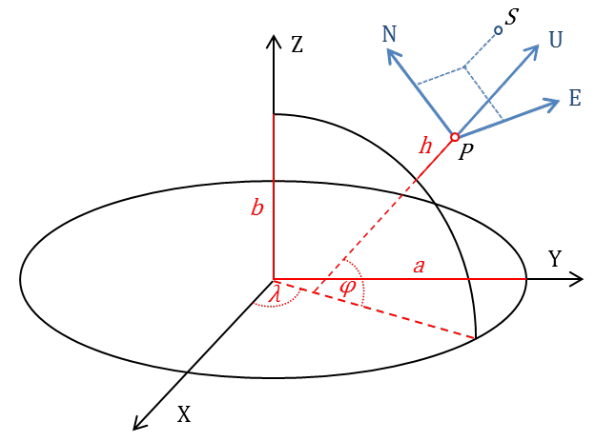
\includegraphics[width=\linewidth]{daisy_local_coord.png}
            \caption{Topocentrikus fel- (U), északi- (N) és keleti (E) irányok a $P$ PS-hez rögzített koordinátarendszerben. $h$ a PS pont ellipszoid feletti magassága, $\lambda$, $\phi$ a ellipszoidi koordináták, $a$ és $b$ az ellipszoid paraméterei, $S$ jelöli a műhold pozícióját.}
        \end{subfigure}
        \hspace{25pt}
        \begin{subfigure}[t]{.49\linewidth}
            \centering
            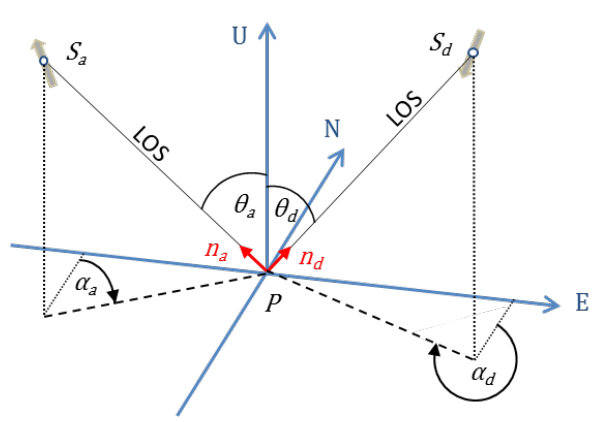
\includegraphics[width=\linewidth]{daisy_schematic.png}
            \caption{Felszálló és leszálló LOS irányok geometriája a lokális PS koordinátarendszerben. $S_{\text{d}}$ és $S_{\text{d}}$ a felszálló és leszálló műholdpozíciók, $\alpha_{\text{a}}$ és $\alpha_{\text{d}}$ az azimut szögek, $\theta_{\text{a}}$ és $\theta_{\text{d}}$ a beesési szögek, $n_{\text{a}}$, $n_{\text{d}}$ a felszálló és leszálló irányú LOS sebességek normálvektorjai.}
        \end{subfigure}
    \caption{A felszálló- és leszálló irányú felvételek geometriája a lokális (UNE) koordinátarendszerben. \cite{Banyai2017}}\label{daisy_schematic}
    \end{figure}
\end{center}

Ahogy azt a \ref{daisy_schematic}. ábrán is látni lehet az $n_{\text{a}}$ és $n_{\text{d}}$ ASC és DSC LOS irányok által kifeszített sík nem esik egybe az UE síkkal, így az U és E sebességkomponenseket csak közelítőleg lehet meghatározni. Itt két tényező tudja a közelítést befolyásolni:
\begin{enumerate}
    \item Ugyan az ASC és DSC LOS sebességek sokkal érzékenyebbek az U és E komponensekre mint az N komponensre, nagy N komponens torzítja U és E komponensek becslését.
    \item Az ASC és DSC LOS sebességek nem ``szimmetrikusak'' (általában $\alpha_{\text{a}} + \alpha_{\text{d}} \ne 2 \pi$ és $\theta_{\text{a}} \ne \theta_{\text{d}}$). Ez zéró N komponens esetén is torzulástokoz az U és E komponensek számított értékeiben.
\end{enumerate}

A feldolgozás menete a következőképpen zajlik:
\begin{enumerate}
    \item A \stamps feldolgozás során elkészült \texttt{master.res} fájlok (ASC és DSC eset) tartalmazzák a műholdak pontos Descartes koordinátáit. A DAISY ezen koordinátapontokra illeszt polinomot az ASC és DSC esetben.
    \item ASC és DSC pontok kiválasztása melyek egy felhasználó által megadott távolságnál közelebb helyezkednek el egymástól.
    \item Csoportok kiválasztása, melyek tartalmaznak legalább egy ASC és egy DSC PS pontot egy felhasználó által megadott sugáron belül.
    \item Minden egyes csoportban fiktív Domináns Szórópont (DP - Dominant Points) koordinátáinak meghatározása. A DP úgy kell meghatározni, hogy annak távolsága a csoporton belül található ASC és DSC PS pontoktól minimális legyen legkisebb négyzetes értelemben.
    \item A DP ASC és DSC LOS sebességeinek meghatározása a csoporton belül található ASC és DSC PS pontokkal. A \texttt{DAISY} az ASC és DSC LOS sebességek súlyozott átlagát számítja ki, a súlyok a távolság négyzetével fordítottan arányosak.
    \item DP-k ASC és DSC LOS paramétereinek kiszámítása a polinomiális pályák felhasználásával.
    \item DP-k pozíciójában a U és E sebességkomponensek becslése.
    \item \textit{Opcionális lépés}: DS pontok kiválasztása, melyek U és E komponensei által alkotott sebességvektor nagysága kisebb egy felhasználó által megadott értéknél.
    \item \textit{Opcionális lépés}: A \stamps-hez hasonlóan, referenciaterület kiválasztása és a referenciaterület átlagos U és E sebességkomponensének levonása a többi kiszámított U és E sebességkomponensekből.
\end{enumerate}

A \texttt{DASIY} program lehetővé teszi az ASC és DSC felvételek kombinálásával a közel U és E komponensek becslését, így a vizsgált terület geodinamikájának pontosabb elemzését.

\chapter{A Kárpát-kanyar és a Csomád-vulkán - geodinamikai alapismeretei}

A Kárpát-kanyar geodinamikai folyamatait Ismail-Zadeh és társai \cite{Matenco2012}, Harangi és társai \cite{Harangi2010, Harangi2014}, van der Hoeven és társai \cite{Hoeven2005} által publikált cikkek alapján mutatom be. Részletes ismertetés megtalálható Ismail-Zadeh és társai \cite{Matenco2012} összefoglaló munkájában.

\section{A Kárpát-kanyar régió}

A Kárpát-kanyar nyugati oldalán valaha aktív vulkáni tevékenység zajlott, melyet egy óceáni lemez szubdukciója táplált. Ennek a vulkáni ívnek a legfiatalabb tagja a Csomád-vulkán. A szubdukció azóta keletebbre húzódott  és ma már az óceáni lemez egésze a földköpenyben található \cite{Matenco2012}, így a vulkáni tevékenység is megszűnt \cite{Harangi2010}.

A kanyarulat másik, keleti, oldalán található a Vrancea-zóna. A Vrancea-zónában sokszor pattannak ki közepes mélységű, nagy erejű földrengések \cite{Matenco2012}, melyek jelentős energia felszabadulásával járnak és gyakran okoznak károkat épületekben. Általánosan elmondható, hogy a kanyarulattól keletre található területek süllyednek, mely a terület alatt zajló szubdukciónak tulajdonítható \cite{Hoeven2005}.

A földrengések a fentebb említett szubdukcióhoz kapcsolódnak. A szubdukció természete a mai napig nem ismert pontosan. Egyes elméletek szerint a Vrancea zóna szeizmicitása a már szubdukálódott és a jelenben a földköpenyben süllyedő óceáni lemezhez köthető. Az, hogy a remanens óceáni lemez csatlakozik-e a kontinentális lemezhez vagy már elvált attól, nyitott kérdés. Egy másik elmélet szerint a kontinentális lemez kontinens-kontinens során megvastagodott és a megvastagodott régió alsó komponense levált a felsőtől és elkezdett szubdukálódni. \cite{Matenco2012}

A kanyari terület alatt szubdukálódó lemez a szeizmikus tomográfia segítségével lehatárolható. A \ref{seism_tomo}. ábra egy P-hullám szeizmikus tomográfia segítségével előállított szelvény látható. A kanyarulattól keletre fekvő terület alatt egy P-hullám anomália található \cite{Matenco2012}. Az anomáliát okozhatja egy már szubdukálódott és földköpenybe alámerülő óceáni lemez. A tomográfia képen az is látható, hogy a feltételezett lemez alsó része éppen leválóban van a lemez sekélyebb részeitől. A szubdukció és a leválás folyamata okozhatja azon földrengéseket, melyek hipocentrumait a fekete pontok jelölik az ábrán.

\begin{figure}
    \centering
    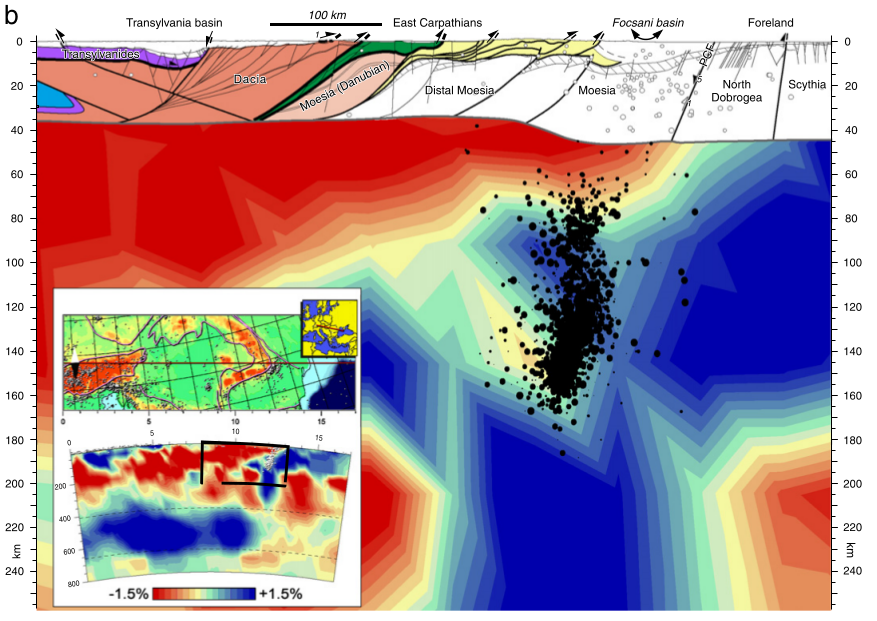
\includegraphics[width=0.75\linewidth]{seism_tomo.png}
    \caption{P-hullám szeizmikus tomográfia szelvény, mely tartalmazza Kárpáti-kanyarulat régiót. A fekete pontok a kipattant földrengések hipocentrumait jelölik.\cite{Matenco2012}}\label{seism_tomo}
\end{figure}

A Vrancea-zónában található földrengések nem okoznak olyan mértékű felszíni elmozdulást, melyet egyetlen interferogramal vizsgálni lehetne, azaz a deformációs fázistag az egyes interferogramok esetén sokkal kisebb, mint az egyéb fázistagok, pl. az atmoszferikus tag; emiatt a térségben végbemenő deformációk interferometrikus elemzése csak az interferogramok idősorelemzésével lehetséges. Továbbá a kicsi deformációs sebesség miatt több éves adatrendszer szükséges ahhoz, hogy meghatározható legyen a deformáció mértéke és sebessége.

A Kárpát-kanyar egy geodinamikailag aktív zóna, melynek megértéséhez a geofizika, geológia és további diszciplínák adatainak, módszereinek alkalmazása szükséges. A radar interferometria egy olyan módszer, mely segíthet a vizsgálati régióban játszódó geodinamikai folyamatok megértésében és a modellezésében.

A Csomád a Kárpát-Pannon vidék legfiatalabb vulkánja (\ref{csomad}. ábra), a Kárpát-kanyarban található vulkáni ívnek a Csomád-hegységnek tagja. A Pannon-térség vulkanizmusának forrása a késő jura és korai kréta időszak között lejátszódott szubdukciója a Neo-Thétisz óceán maradványának \cite{Matenco2012}. A szubdukálódó óceáni litoszféra által létrehozott vulkánosság aktív régiója egyre keletebbre és egyben délebbre tolódott követve a szubdukciós zónát \cite{Harangi2014}. Ezen vulkáni láncolat utolsó és egyben legfiatalabb tagja a Csomád-vulkán.

\begin{figure}[H]
    \centering
    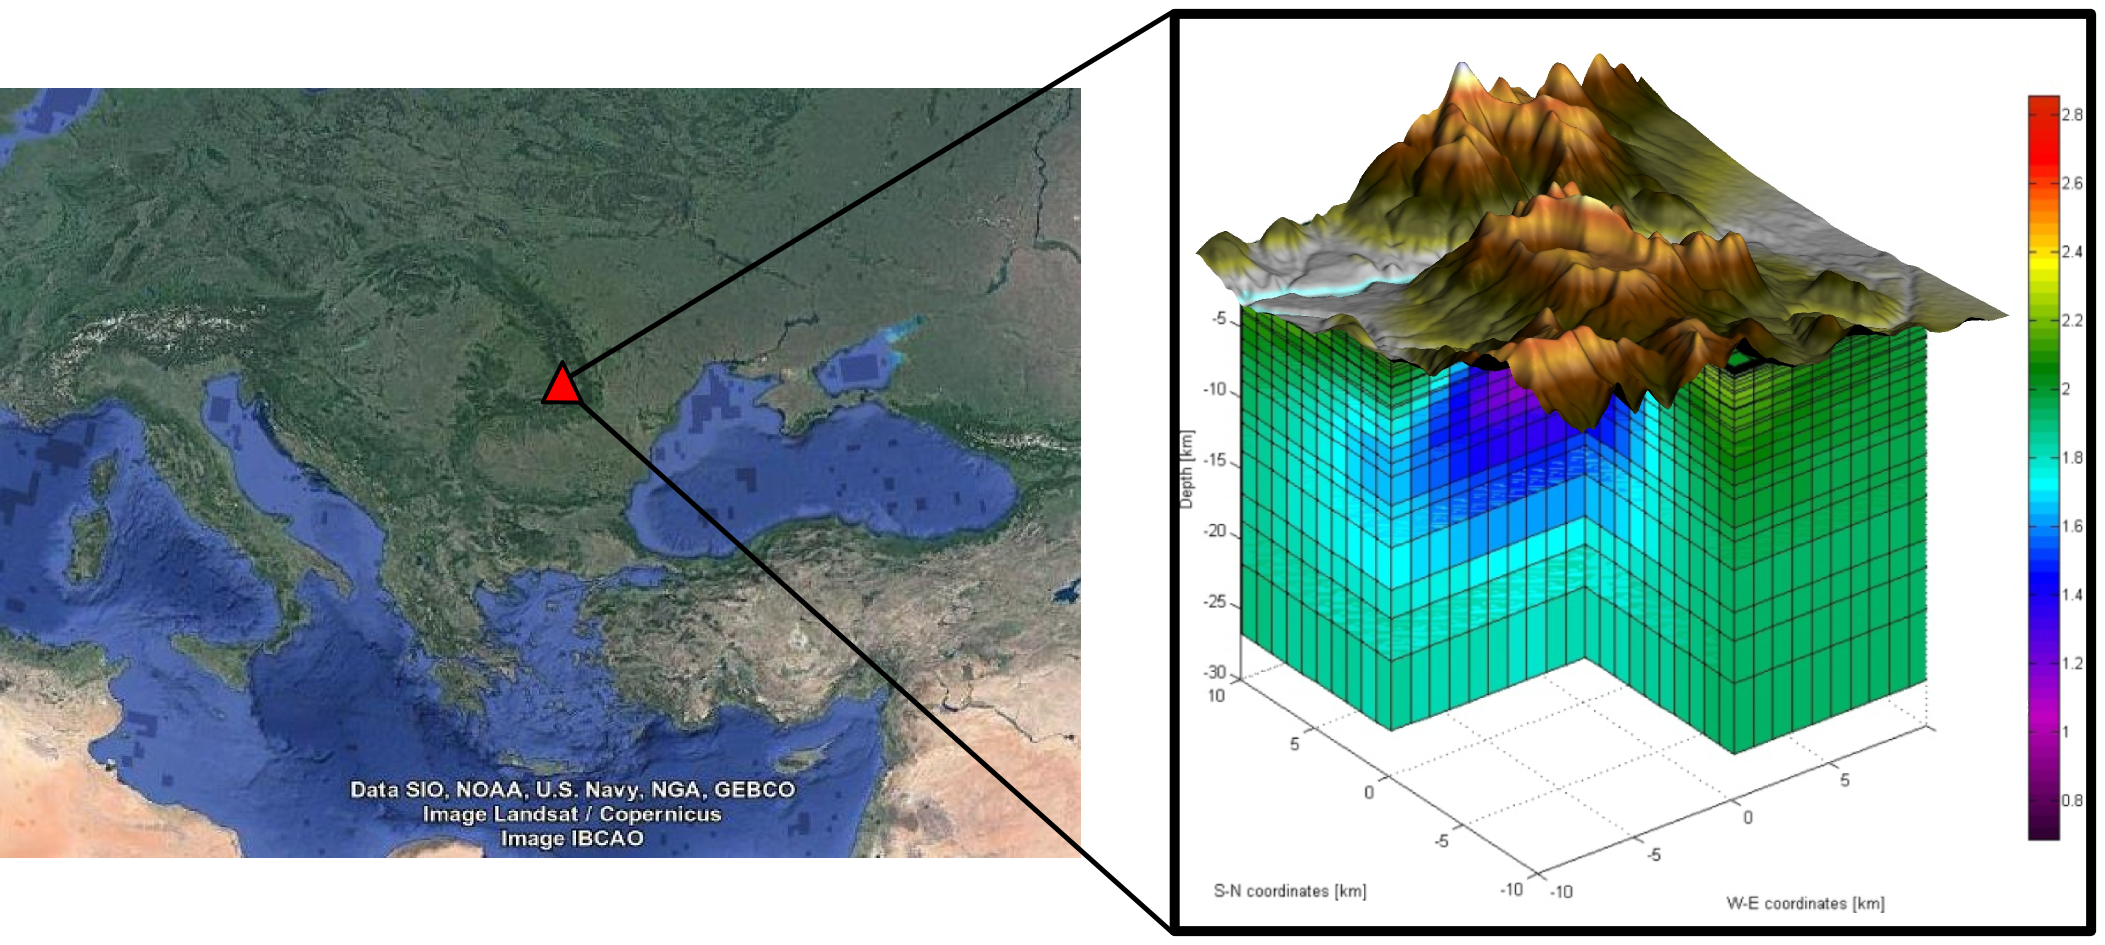
\includegraphics[width=0.85\linewidth]{google_earth_csomad_harangi.png}
    \caption{A Csomád-vulkán elhelyezkedése a Kárpát-kanyar területén, a baloldali képen. Jobbra a vulkán domborzati modellje látható, alatta a magnetotellurikus mérések alapján inverzióval meghatározott fajlagos ellenállás értékek \cite{Harangi2014}. A színskála logaritmikus, az ellenállás értékek dimenziója $\si{\ohm\meter}$}.\label{csomad}
\end{figure}

A vulkán nagyjából 30 000 évvel ezelőtt volt aktív \cite{Harangi2010}. Magnetotellurikus vizsgálatok \cite{Harangi2014} és szeizmikus tomográfia \cite{Popa2012} segítségével kimutatták, hogy egy alacsony fajlagos vezetőképességgel és szeizmikus hullámterjedési sebességgel rendelkező anomália található a vulkán alatt. \cite{Harangi2014} szerint a fenti eredmények arra utalnak, hogy a Csomád alatt egy parciálisan olvadt zóna található, melyet újra aktivizálhat egy magmabehatolás, ami a Csomád-vulkán kitöréséhez vezethet.

\section{A Kárpát-kanyar régiójában végzett geodéziai mérések}\label{GNSS}

Az itt zajló tektonikai folyamatok modellezése igazi kihívás, mivel az elmozdulások, deformációk nagy mélységekben történnek, a nagy földrengéseket leszámítva csekély felszíni indikációval. A deformációk azonban fontos peremfeltételt jelentenek a különböző kvantitatív, numerikus modellezésen alapuló vizsgálatokhoz. Több, nemzetközi összefogásban végzett kísérlet történt ismételt GNSS mérések alapján az elmozdulások meghatározására.

Két GNSS mérési kampányt mutatok be és összehasonlítom a mérési adatokból számított vertikális és horizontális sebességtereket. van der Hoeven és társai \cite{Hoeven2005} 25 kihelyezett GNSS állomás, 13 kampány során regisztrált méréseit foglalja össze. Az állomások 1997 és 2004 között végeztek méréseket. Schmitt és társai \cite{Schmitt2007} 14 GNSS kampány méréseit foglalja össze, 1995-től 2006-ig tartó időintervallumban. A méréseket változó állomásszámmal végezték el. A két cikkben \cite{Hoeven2005, Schmitt2007} bemutatott vertikális sebességek a \ref{gps_vertical}. ábrán láthatóak, míg a horizontális sebességek a \ref{gps_horizontal}. ábrán.

\begin{center}
    \begin{figure}[H]
        \begin{subfigure}[t]{.40\linewidth}
            \centering
            \includegraphics[height=10cm]{hoeven_gps_with_graticule.png}
            \caption{GNSS állomások által mért vertikális deformációs sebességek. A nyilak az állomásokon mért sebességeket jelölik, a hibaellipszisek a 95\%-os konfidencia intervallumot. A színskála az interpolált vertikális sebességértékeket jelöli $\text{mm}/\text{év}$ egységekben. \cite{Hoeven2005}}
        \end{subfigure}
        \hspace{25pt}
        \begin{subfigure}[t]{.40\linewidth}
            \centering
            \includegraphics[height=10.25cm]{schmitt_vertical.png}
            \caption{GNSS állomások által mért vertikális deformációs sebességek. A nyilak az állomásokon mért sebességeket jelölik. A színskála az interpolált vertikális sebességértékeket jelöli $\text{m}/\text{év}$ egységekben. \cite{Schmitt2007}}
        \end{subfigure}
        \caption{van der Hoeven és társai, Schmitt és társai \cite{Hoeven2005, Schmitt2007} által GNSS mérések alapján összeállított vertikális sebességmező a Kárpát-kanyar területén.}\label{gps_vertical}
    \end{figure}
\end{center}

\begin{center}
    \begin{figure}[H]
        \begin{subfigure}[t]{.4\linewidth}
            \centering
            \includegraphics[height=10cm]{hoeven_horizontal.png}
            \caption{GNSS állomások által mért horizontális deformációs sebességek. A piros nyilak az állomások sebességeit jelölik, a hibaellipszisek a 95\%-os konfidencia intervallumot. A fekete nyilak az interpolált sebességeket reprezentálják. Az Eurázsiai lemezhatárok sebessége zéró. \cite{Hoeven2005}}
        \end{subfigure}
        \hspace{25pt}
        \begin{subfigure}[t]{.4\linewidth}
            \centering
            \includegraphics[height=10.25cm]{schmitt_horizontal.png}
            \caption{GNSS állomások által mért horizontális deformációs sebességek. A piros nyilak az állomások sebességeit jelölik, a hibaellipszisek a 95\%-os konfidencia intervallumot. A fekete nyilak az interpolált sebességeket reprezentálják. \cite{Schmitt2007}}
        \end{subfigure}
        \caption{van der Hoeven és társai, Schmitt és társai \cite{Hoeven2005, Schmitt2007} által GNSS mérések alapján összeállított horizontális sebességmező a Kárpát-kanyar területén.}\label{gps_horizontal}
    \end{figure}
\end{center}

Mind a vertikális, mind a horizontális sebességkomponensek esetén kevés olyan területet találunk, ahol egyeznének a mért eredmények, annak ellenére, hogy a mérések nagyjából egyazon időintervallumban készültek. Közelítőleg egy irányba mutatnak a GNSS sebességvektorok az É \ang{45}, K \ang{27} körüli területen (\ref{gps_vertical}. ábra) a vertikális, és É \ang{45.5}, K \ang{26.5} szomszédságában a horizontális sebességek esetén (\ref{gps_horizontal}. ábra).

Az általam vizsgált terület (É\ang{46}, K\ang{26}) környékén a horizontális sebességek van der Hoeven és társai \cite{Hoeven2005} szerint déli irányú mozgást mutatnak, kis keleti irányú komponenssel. Schmitt és társai \cite{Schmitt2007} által vizsgált területen a horizontális sebességkomponensek értéke kicsi, de szintén főleg déli- kissé keleti irányú mozgást mutat. A sebességek nagysága nem haladja meg az $1.5 \text{mm}/\text{év}$-et. A vertikális sebességek iránya a két GNSS mérés esetén egyezik a nagyságrendben sincs jelentős eltérés (emelkedés sebessége: $\approx 1-3 \text{mm}/\text{év}$, süllyedés sebessége: $2-3 \text{mm}/\text{év}$ mindkét GNSS mérés esetében).

A van der Hoeven és társai és Schmitt és társai \cite{Hoeven2005, Schmitt2007} által publikált pontos GNSS adatok nem álltak rendelkezésre az Intézet részére, így nem állt módomban a fentinél pontosabb összehasonlítást végezni. Elmondható azonban, hogy a GNSS hálózatok egészét tekintve jelentős elmondások tapasztalhatóak a van der Hoeven és társai és Schmitt és társai \cite{Hoeven2005, Schmitt2007} által kiszámított 3D sebesség mező között.

Annak érdekében, hogy a régió geodinamikai folyamataira pontos magyarázatot lehessen adni szükség lenne pontos és hiteles felszíni deformációs idősorokra és sebességekre. Az InSAR technológia egy független módszer, amely hozzájárulhat más geodéziai módszerrel mért sebességek értelmezéséhez is, továbbá az InSAR, koherens interferogramok esetén, sokkal jobb térbeli felbontást és lefedettséget biztosít, így általában nem szükséges interpoláció.

\chapter{Az archív Envisat felvételek feldolgozása}

A Geodéziai és Geofizikai Intézet (GGI) az Európai Űrügynökség (ESA - European Space Agency) Scientific Project Proposal CAT-1 30142 pályázatának keretében jutott hozzá archív Envisat SAR felvételekhez. Az adatrendszer 23 felszálló és 32 leszálló irányú felvételt tartalmaz, melyek úgy kerültek kiválasztásra, hogy átfedésben legyenek a korábbi GNSS mérések időpontjaival, így a 2002-2010 időintervallumot fedik le.

Az Envisat egy alacsony pályán keringő, földmegfigyelő műhold volt, az ERS műholdak utódja, melyet az ESA bocsájtott fel 2002-ben.  A műhold C sávban működő ($\lambda = \SI{5.6}{\centi\meter}$) ASAR (Advenced Synthetic Aperture Radar) antennája névlegesen 35 naponta készített ugyanarról a területről felvételeket, azonban különböző hibák miatt több esetben ennél nagyobb  időtartam van egy-egy egymást követő felvétel között a pályázatban beszerzett adatbázisban. A műholdon összesen 10 műszer működött (\url{https://earth.esa.int/web/guest/missions/esa-operational-eo-missions/envisat/instruments}). Az Envisat misszió 2012. április 8.-án ért véget miután váratlanul megszakadt a kapcsolat a műholddal. \url{https://earth.esa.int/web/guest/missions/esa-operational-eo-missions/envisat}

A felvételek feldolgozásához több programcsomagot felhasználtam. A felhasznált programcsomagokat a \ref{programs} fejezetben foglalom össze, az előfeldolgozás menetét pedig a \ref{processing} fejezetben írom le.

\section{Az Envisat felvételek}

A GGI az ESA-tól nyers SAR felvételeket kapott. A felvételeket előfeldolgozásáról a \ref{processing}. fejezetben lehet olvasni. Az előfeldolgozás során a felvételeket fókuszálni kell, koregisztrálni a mesterképhez, SLC képeket készíteni a SAR képekből, majd az előállítani az interferogramokat. Végül interferogramokból ki kell vonni a topográfiai fázistagokat.

A \ref{psi_asc}. táblázatban a felszálló, a \ref{psi_dsc}. táblázatban pedig a leszálló irányból készült interferogramok mesterképtől számított időbeli és térbeli bázisvonalai láthatóak PSI módszer esetén.

\begin{table}[H]
    \begin{center}
        \begin{tabular}{m{3cm} c c || m{3cm} c c} \toprule
            Szolgafelvételek készítésének időpontja & $B_{\perp} [\si{\meter}]$ & $\Delta T$ (nap) & Szolgafelvételek készítésének időpontja & $B_{\perp} [\si{\meter}]$ & $\Delta T$ (nap)\\ \midrule
            2002.12.07. & 206.5 & -595 & 2005.08.13 & 910.2 & 385 \\
            2003.04.26 & -542.2 & -455 & 2005.11.26 & 571.1 & 490 \\
            2003.07.05 & -77.8 & -385 & 2006.06.24 & -512.6 & 700 \\
            2003.09.13 & 17 & -315 & 2006.07.29 & -525.8 & 735 \\
            2004.03.06 & 78.2 & -140 & 2007.02.24 & 73.8 & 945 \\
            2004.07.24. & 0 & 0 & 2007.06.09 & 89.5 & 1050 \\
            2004.08.28 & 458.8 & 35 & 2007.08.18 & 531.7 & 1120 \\
            2004.11.06 & 42.1 & 105 & 2008.08.02 & 219.3 & 1470 \\
            2005.01.15 & -356.4 & 175 & 2008.10.11 & -64.3 & 1540 \\
            2005.02.19 & 782.3 & 210 & 2009.04.04 & 631.9 & 1715 \\
            2005.06.04 & 371 & 315 & 2010.05.29 & 294.1 & 2135 \\ \bottomrule
        \end{tabular}
        \caption{Felszálló irányú interferogramok bázisvonal értékei. A táblázatban a mesterképhez viszonyított merőleges térbeli, $B_{\perp}$ és időbeli, $\Delta T$, bázisvonalak láthatóak. A mesterkép bázisvonalai nullák.}\label{psi_asc}
    \end{center}
\end{table}

\begin{table}[H]
    \begin{center}
        \begin{tabular}{m{3cm} c c || m{3cm} c c} \toprule
            Szolgafelvételek készítésének időpontja & $B_{\perp} [\si{\meter}]$ & $\Delta T$ (nap) & Szolgafelvételek készítésének időpontja & $B_{\perp} [\si{\meter}]$ & $\Delta T$ (nap)\\ \midrule
            2002.11.21 & 856.6 & -1610 & 2006.06.08 & -261.6 & -315 \\
            2003.06.19 & -47.2 & -1400 & 2006.07.13 & 948 & -280 \\
            2003.11.06 & -839.6 & -1260 & 2006.09.21 & -831.8 & -210 \\
            2004.01.15 & 299.3 & -1190 & 2007.02.08 & -74.5 & -70 \\
            2004.03.25 & 1197.7 & -1120 & 2007.04.19 & 0 & 0 \\
            2004.06.03 & 529.9 & -1050 & 2007.09.06 & 463.5 & 140 \\
            2004.10.21 & 672 & -910 & 2007.11.15 & 469.6 & 210 \\
            2004.12.30 & 496.5 & -840 & 2008.02.28 & -173.9 & 315 \\
            2005.02.03 & -123.5 & -805 & 2008.09.25 & -165.5 & 525 \\
            2005.04.14 & 269.8 & -735 & 2009.02.12 & 53.4 & 665 \\
            2005.07.28 & 508.6 & -630 & 2009.04.23 & -32.3 & 735 \\
            2005.09.01 & 853.8 & -595 & 2009.05.28 & 265.7 & 770 \\
            2005.11.10 & 674.5 & -525 & 2010.04.08 & 473.4 & 1085 \\
            2005.12.15 & 321.7 & -490 & 2010.06.17 & 352.6 & 1155 \\
            2006.02.23 & -78.8 & -420 & 2010.07.22 & -145.6 & 1190 \\
            2006.03.30 & -885 & -385 & 2010.09.30 & 612.7 & 1260 \\ \bottomrule
        \end{tabular}
        \caption{Leszálló irányú interferogramok bázisvonal értékei. A táblázatban a mesterképhez viszonyított merőleges térbeli, $B_{\perp}$ és időbeli, $\Delta T$, bázisvonalak láthatóak. A mesterkép bázisvonalai nullák.}\label{psi_dsc}
    \end{center}
\end{table}

\section{A feldolgozáshoz felhasznált programcsomagok}\label{programs}

A nyers SAR felvételek feldolgozásához felhasznált programcsomagokat a \ref{programs_table}. táblázat tartalmazza. A \texttt{ROI\_PAC} program végezte el a nyers SAR felvételek fókuszálását, az SLC felvételek és az interferogramok pedig a \texttt{DORIS} programmal készültek. Szintén a \texttt{DORIS} program végezte el a topográfiai korrekciót. A \stamps programmal történt az interferogramok idősorelemzése, mely felhasználja a \texttt{SNAPHU} programot a fáziskicsomagolásnál. A \texttt{DAISY} program integrálta az ASC és DSC felvételeket és számította ki a vertikális- és kelet-nyugati sebességkomponenseket.

\begin{table}[H]
    \begin{center}
        \begin{tabular}{p{6cm} p{10cm}} \toprule
            Programcsomag neve & Leírás \\ \midrule
            \texttt{ROI\_PAC} \cite{roi_pac} & nyers SAR felvételek és egyéb kiegészítő adatok (DEM, precíz pályák, kalibrációs fájlok) felhasználásával származtatott SLC képeket készít \\[12pt]
            \texttt{DORIS} InSAR Processor \cite{doris} & SLC felvételből interferometrikus produktumok készítése (DEM, elmozdulás térkép) \\[12pt]
            \stamps \cite{Hooper2012} & interferogramok idősorelemzésével átlagos műhold LOS felszíni elmozdulási sebességeket és deformációs idősorokat készít \\[12pt]
            \texttt{SNAPHU} \cite{snaphu} & 2D-s fáziskicsomagoló algoritmus \\[12pt]
            \texttt{DAISY} \cite{Banyai2016} & ASC és DSC LOS sebességek integrálásával vertikális és kelet-nyugat irányú sebességkomponenseket számít ki. \\ \bottomrule
        \end{tabular}
        \caption{A nyers Envisat SAR felvételek feldolgozásához felhasznált programok.}\label{programs_table}
    \end{center}
\end{table}

\section{Az előfeldolgozás menete}\label{processing}

A \stamps programcsomag tartalmazza a megfelelő \texttt{bash} nyelvben megírt parancsokat, melyek meghívják a megfelelő \texttt{ROI\_PAC}, \texttt{Doris} parancsokat és scripteket, majd elvégzik az előfeldolgozást. Az \ref{processing_flowchart}. ábra mutatja be hogyan kell a nyers SAR felvételeket az idősorelemzéshez előkészíteni.

\begin{figure}[H]
    \centering
    \begin{tikzpicture}[node distance=2cm]
        % Place nodes
        \node [startstop, align=center] (raw_in) {Nyers\\SAR felvételek};
        \node [process, below of=raw_in] (choose_crop) {Mesterkép előkészítése};
        \node [io, align=center, right of=choose_crop, xshift=12.5em] (choose_crop_in) {mesterkép,\\terület kiválasztása};
        \node [process, below of=choose_crop] (make_slcs) {SLC-k elkészítése};
        \node [process, align=center, below of=make_slcs] (master_timing) {(step\_master\_orbit\_ODR)\\step\_master\_timing\\make\_orbits\\make\_coarse};
        \node [process, below of=master_timing, xshift=-5em, yshift=-1em] (make_coreg) {make\_coreg};
        \node [process, below of=master_timing, xshift=5em, yshift=-1em] (make_dems) {make\_dems};
        \node [io, left of=master_timing, align=center, xshift=-7.5em] (DEM_in) {DEM,\\precíz\\pályaadatok};
        \node [decision, align=center, below of=master_timing, yshift=-7.5em] (check_baselines) {Bázisvonalak,\\koherencia\\ellenőrzése};
        \node [io, align=center, right of=check_baselines, xshift=12.5em] (baseline_no) {új mester\\választása};
        \node [process, align=center, below of=check_baselines, yshift=-1em, yshift=-3em] (make_resample) {make\_resample\\make\_ifgs\\step\_geo};,
        \node [process, below of=make_resample] (mt_prep) {mt\_prep};
        \node [startstop, below of=mt_prep] (stamps) {\stamps};
        % Draw arrows
        \draw [arrow] (raw_in) -- (choose_crop);
        \draw [arrow] (choose_crop) -- (make_slcs);
        \draw [arrow] (choose_crop_in) -- (choose_crop);
        \draw [arrow] (make_slcs) -- (master_timing);
        \draw [arrow] (baseline_no) -- (choose_crop_in);
        \draw [arrow] (master_timing) -- (make_dems);
        \draw [arrow] (master_timing) -- (make_coreg);
        \draw [arrow] (make_coreg) -- (check_baselines);
        \draw [arrow] (make_dems) -- (check_baselines);
        \draw [arrow] (DEM_in) -- (master_timing);
        \draw [arrow] (check_baselines) -- node [anchor=south] {Nem fogadjuk el} (baseline_no);
        \draw [arrow] (check_baselines) -- node [anchor=east] {Elfogadjuk} (make_resample);
        \draw [arrow] (make_resample) -- (mt_prep);
        \draw [arrow] (mt_prep) -- (stamps);
    \end{tikzpicture}
    \caption{A nyers SAR adatok előfeldolgozásának menete a \stamps feldolgozás előkészítéséhez.}\label{processing_flowchart}
\end{figure}

Első lépésként ki kell választani a mesterképet és a mesterképen belül a vizsgálandó területet. A terület kiválasztásánál figyelni kell arra, hogy a kiválasztott terület minden más képen is szerepeljen. Ha nem rendelkezünk semmilyen előismerettel a felvételek minőségéről, akkor érdemes az idősor közepéről választani egy képet, melyen nem található hótakaró. A feldolgozás során később kiadható a \code{master\_select} parancs, melynek segítségével új mesterkép választható.

Miután kiválasztottuk a mesterképet le kell határolni a mesterképen a vizsgálandó területet. A terület kijelölést, úgy kell elvégezni, hogy a kijelölt terület minden szolgaképen szerepeljen. A kijelölt terület pixelhatárait a \texttt{master\_crop.in} fájlba kell regisztrálni, majd futtatni a \code{step\_master\_setup} parancsot. A \code{make\_slcs\_xxx} parancs kiadása után elkészülnek a SLC képek (xxx = envi, ers,\dots felvételek típusától függően).

Ha rendelkezésre állnak precíz pályaadatok futtatni kell a \code{step\_master\_orbit\_ODR} parancsot. Majd először a \texttt{timing.dorisin} sablon fájlba a helyes DEM paramétereket kell betáplálni (DEM kiterjedése, adattípus, teljes útvonal a DEM fájlhoz) majd egymás után lehet futtatni a \code{step\_master\_timing}, \code{make\_orbits}, \code{make\_coarse} és a \code{make\_coreg} parancsokat. A \code{step\_master\_timing} kiszámítja a mesterkép ``időzítési'' hibáját, mely a georeferáláshoz és a pontos DEM pozíciók kiszámításához kell. A \code{make\_orbits} a precíz műholdpályaadatokat állítja elő a mester- és szolgaképekhez. A \code{make\_coarse} és a \code{make\_coreg} a szolgaképek koregisztrációját végzi el a mesterképhez.  Az eljárás során a $B_{\perp} < \SI{100}{\meter}$-el rendelkező képpárokat regisztrálja össze. Ha egy szolga- és mesterkép között nagyobb a merőleges bázisvonal különbség az algoritmus a szolgaképet 3 ``közelebbi'' szolgaképhez regisztrálja. A \code{make\_coreg} parancs mellett futhat a \code{make\_dems} parancs is, mely a topográfiai korrekciót számítja ki.

\begin{sloppypar}
Mindezek után le lehet futtatni a \code{master\_select} parancsot, mely kiszámítja az interferogramok stack koherenciáját minden lehetséges esetre. A \code{grep Bperp */coreg.out} parancs pedig a mesterképtől számított merőleges bázisvonalakat nyomtatja ki a parancssorra. Ha úgy döntünk, hogy másik mesterképet választunk az új mesterkép \texttt{master\_crop.in} fájl szerkesztése után a \code{step\_master\_orbit\_ODR} parancs kiadásától folytathatjuk.
\end{sloppypar}

Ha megtartjuk a mesterképet a \code{make\_resample} (szolgaképek újramintavételezése a mesterképhez), \code{make\_ifgs} (interferogramok elkészítése), \code{step\_geo} (georeferálás elvégzése egy szolgaképre) parancsokkal folytatjuk.

Végül az \code{mt\_prep} parancs előkészíti az interferogramokat a \stamps feldolgozásra. A parancs kiválogatja az előzetes PS pixeleket (\ref{stamps}. fejezet) és a képeket több ún. \textit{patch}-re bontja szét, annak érdekében, hogy a különböző patch-eket egyenként lehessen feldolgozni és a feldolgozást végző számítógép memóriája ne teljen be. Ezután a \stamps programba betöltve az adatokat elvégezhető a PSI idősorelemzés.

Ha SBAS módszerrel kívánjuk feldolgozni az adatainkat, akkor először a \texttt{Matlab}-ban el kell készíteni az SBAS hálózatot. A hálózatot egy függvény generálja le, melynek meg lehet adni paramétereket (minimális koherencia, maximális időbeli és térbeli bázisvonal), melyek alapján a függvény elvet bizonyos interferogramokat. Az SBAS hálózatot egyszerű szövegszerkesztő programmal is meg lehet változtatni. Ezután a \code{make\_small\_baselines} parancs legyártja az interferogramokat egy külön mappába és ott el lehet végezni a \stamps feldolgozást.

\section{A \stamps idősorelemzés}

A felvételeket először a PSI módszerrel próbáltam feldolgozni. A PSI módszer esetében az interferogramok minden esetben egy szolga és a mesterkép felhasználásával készülnek el. Ez a módszer igen nagy tér- és időbeli bázisvonalakat eredményezett, melyeket \ref{psi_asc}. és \ref{psi_dsc}. táblázatban lehet megtekinteni. Az interferogramokban szinte csak a városi területeken maradt meg a koherencia, ami azt eredményezte, hogy csak néhány elszeparált csoportban volt képes a program PS pixeleket találni. A PS pixelek térbeli elhelyezkedésének inhomogenitása a fáziskicsomagolás lépését nehezíti meg. Ugyan a fáziskicsomagolás lépésénél a program képes a kicsomagolt fázisértékek előállítására, ám azok szinte minden esetben hibás értékkel rendelkeznek, mivel a PS pixelek közötti nagy távolságok miatt a fázisugrásokat nem volt képes a kicsomagoló algoritmus helyesen feloldani.

A PSI módszerrel nem sikerült a megfelelő PS térbeli eloszlást elérni és a PS-ek esetén a feldolgozás nem vezetett megbízható eredményekre, ezért a PSI módszer helyett az SBAS módszerrel készítettem el az interferogramokat. A felszálló és leszálló irányú felvételekből alkotott SBAS interferogram hálózat a \ref{asc_dsc_sbas}. ábrán látható.

A bázisvonalak az SBAS módszer alkalmazásával csökkenthetőek, így stack koherencia növelhető és az SBAS interferogram hálózatban található redundáns ``hurkok'' (pl. \ref{asc_dsc_sbas}. ábra (a) ábra 9-10-11 interferogram által alkotott hurok) segítségével a fáziskicsomagolás hibája is becsülhető. Ugyanis, ha egy ``hurkon'' belül összeadjuk a fázisértékeket akkor visszatérve a kiinduló képhez a fázisértékek összege nulla kell, hogy legyen. A nem nulla érték kicsomagolási hibára utal.

A \stamps feldolgozás előtt létrehoztam egy  a program által automatikusan legenerált SBAS hálózatot, mind a fel- és leszálló irányú képek esetén, mely a \ref{asc_dsc_sbas_full}. ábrán látható. Ugyan az SBAS módszer kisebb bázisvonalakat eredményezett, mind térben és időben, képmegjelenítő programmal megvizsgálva az interferogramokat, megállapítottam, hogy jelentős részuk így is inkoherens maradt. A koherens interferogramok esetén is csak bizonyos területeken maradt meg a koherencia és ezen koherens területeknek képről képre változik a pozíciójuk. A demonstráció végett bemutatok egy inkoherens (a) és egy koherens (b) interferogramok a \ref{incoh_coh}. ábrán.

\begin{center}
    \begin{figure}[H]
        \begin{subfigure}[t]{.49\linewidth}
            \centering
            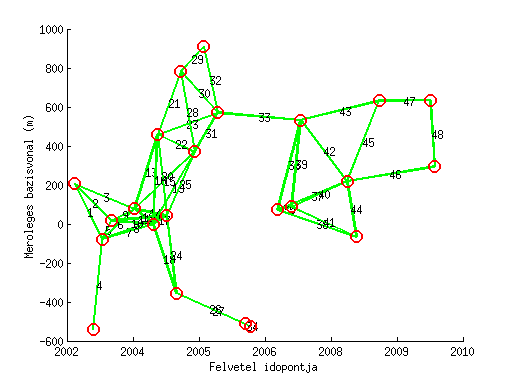
\includegraphics[width=\linewidth]{asc_sbas_full.png}
            \caption{Felszálló irányú felvételekből \stamps program által kialakított SBAS interferogram hálózat.}
        \end{subfigure}
        \hspace{10pt}
        \begin{subfigure}[t]{.49\linewidth}
            \centering
            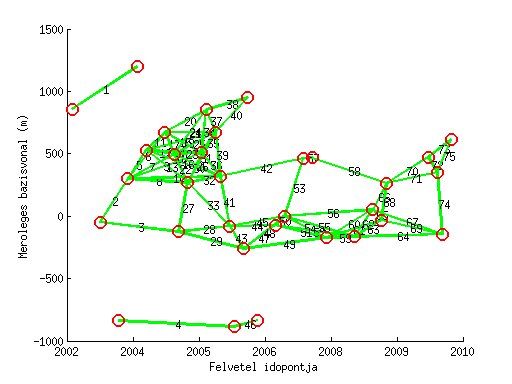
\includegraphics[width=\linewidth]{dsc_sbas_full.png}
            \caption{Leszálló irányú felvételekből \stamps program által kialakított SBAS interferogram hálózat.}
        \end{subfigure}
    \caption{A \stamps program által automatikusan generált SBAS hálózat leszálló és felszálló irányú, felvételekre. A \stamps koherencia és bázisvonalak alapján vet el bizonyos interferogramokat. Nem kerülnek be az interferogramok a hálózatba, ha koherenciájuk kisebb mint 0.5, ha merőleges térbeli bázisvonaluk nagyobb mint $\SI{1070}{\meter}$ vagy ha térbeli bázisvonaluk nagyobb mint 1500 nap. Ezen kritériumfeltételek a felhasználó által is változtathatóak.}\label{asc_dsc_sbas_full}
    \end{figure}
\end{center}

\begin{center}
    \begin{figure}[H]
        \begin{subfigure}[t]{.4\linewidth}
            \centering
            \scalebox{1}[-1]{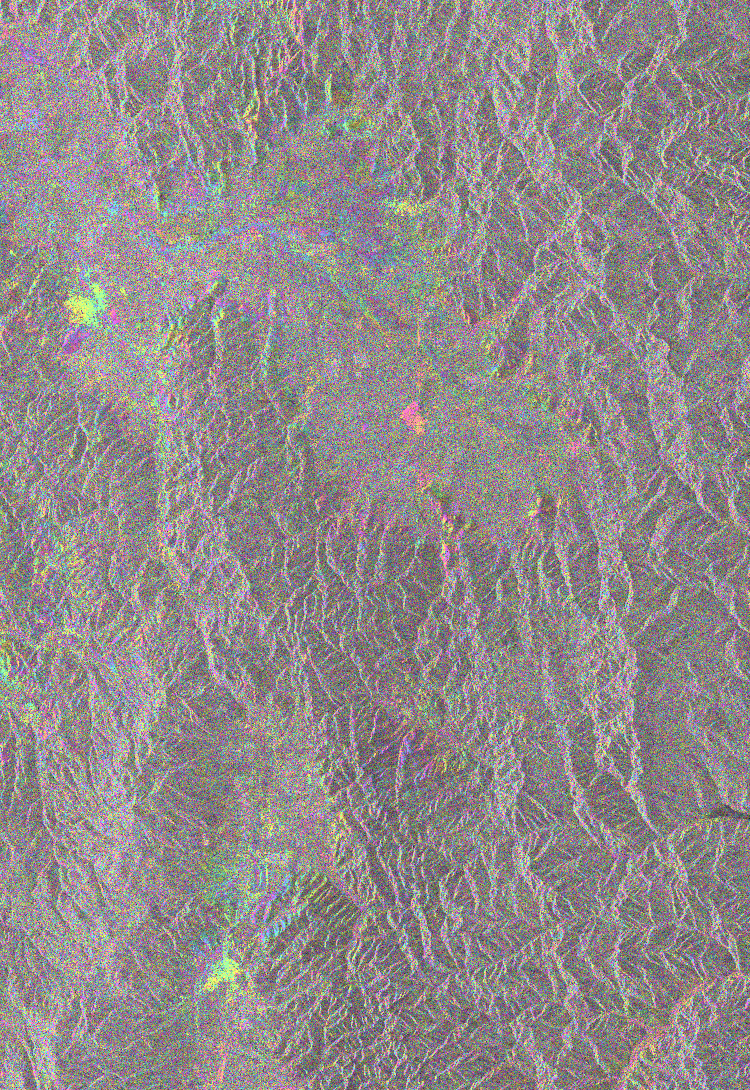
\includegraphics[width=0.8\linewidth]{ifg_bad.png}}
            \caption{Inkoherens interferogram, a fázisváltozás a két felvétel, 2003.09.13.-2004.03.06. ($\Delta T= 175$ nap, $B_{\perp} = \SI{61}{\meter}$) között véletlenszerű. Némi koherencia tapasztalható a városi környezetben.}
        \end{subfigure}
        \hspace{50pt}
        \begin{subfigure}[t]{.4\linewidth}
            \centering
            \scalebox{1}[-1]{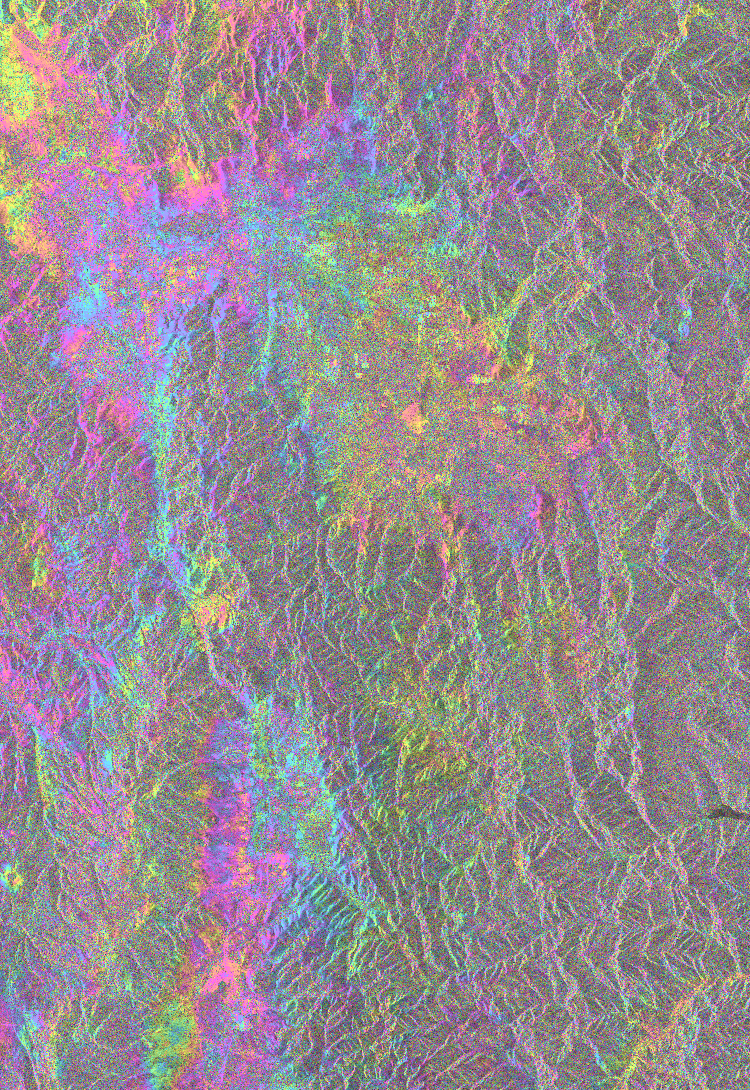
\includegraphics[, width=0.8\linewidth]{ifg_good.png}}
            \caption{Koherens interferogram, a felvétel időpontjai:
            2003.09.13.-2004.03.06. ($\Delta T= 70$ nap, $B_{\perp} = \SI{95}{\meter}$). A koherens fázisértékeket az atmoszferikus tag dominálja.}
        \end{subfigure}
    \caption{Inkoherens (a) és koherens (b) interferogram. A képen szürke színskálával a SAR amplitúdó a topográfiát rajzolja ki, a lila-zöld színskála pedig a fázisértékeket.}\label{incoh_coh}
    \end{figure}
\end{center}

Érdemes megfigyelni, ugyan a koherens interferogram nagyobb merőleges (térbeli) bázisvonallal rendelkezik, mint az inkoherens, mégis nagyobb területen megmarad a koherencia, mint az inkoherens esetben. Ez minden bizonnyal a rövidebb időbeli bázisvonalnak köszönhető (koherens kép: $\Delta T= 70$ nap, inkoherens kép: $\Delta T= 175$ nap). A vizsgált terület esetén az inkoherencia fő okozója az időbeli dekorreláció, melyet az atmoszféra változása és a vegetáció jelenléte okoz. A koherens képen jól látszik, hogy a koherencia elveszik az erősen vegetált, erdős, dombos területeken.

Az automatikusan generált interferogramok halmazából, olyan koherens interferogramokat válogattam össze, melyek területének nagy része koherens pixelekkel van lefedve, jellegüket tekintve hasonlítanak a \ref{incoh_coh}. ábra látható koherens interferogramhoz. A koherens interferogramokból összeállított SBAS hálózatot kiegészítettem kedvezőtlenebb felvételi geometriájú interferogramokkal úgy, hogy a teljes időtartomány vizsgálható legyen, a hálózatban legyenek redundáns ``hurkok'' és a koherens interferogramok összeköttetésben legyenek más interferogramokon keresztül a mesterképpel. Az így elkészült SBAS hálózat fel- és leszálló képek esetén a \ref{asc_dsc_sbas}. ábrán látható. A válogatott interferogramok bázisvonal értékeit a \ref{sbas_asc}. és \ref{sbas_dsc}. táblázatok tartalmazzák leszálló és felszálló képek esetén.

\begin{center}
    \begin{figure}[H]
        \begin{subfigure}[t]{.49\linewidth}
            \centering
            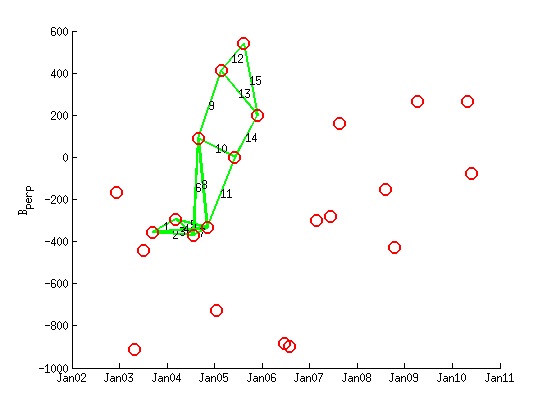
\includegraphics[width=\linewidth]{asc_sbas_select.png}
            \caption{Felszálló irányú felvételekből kialakított SBAS interferogram hálózat.}
        \end{subfigure}
        \hspace{10pt}
        \begin{subfigure}[t]{.49\linewidth}
            \centering
            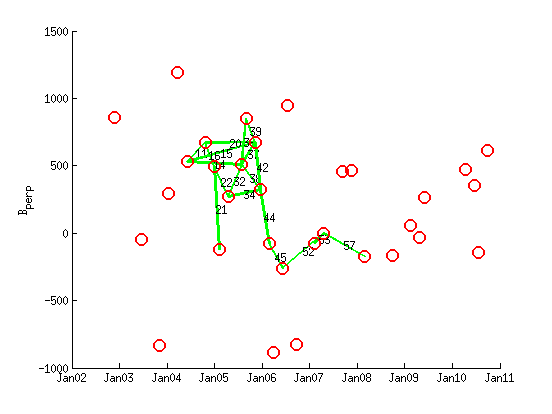
\includegraphics[width=\linewidth]{dsc_sbas_select.png}
            \caption{Leszálló irányú felvételekből kialakított SBAS interferogram hálózat.}
        \end{subfigure}
    \caption{SBAS hálózat leszálló- és felszálló irányú, szelektált interferogramok esetén.}\label{asc_dsc_sbas}
    \end{figure}
\end{center}

\begin{table}[H]
    \begin{center}
        \begin{tabular}{p{2cm} c r r} \toprule
            Interferogram sorszáma & Felvételek & $B_{\perp} [\si{\meter}]$ & $\Delta T$ (nap) \\ \midrule
            1 & 2003.07.05. - 2003.09.13. & 95 & -70 \\
            2 & 2003.07.05. - 2004.07.24. & 78 & -385 \\
            3 & 2003.09.13. - 2004.07.24. & -17 & -315 \\
            4 & 2004.03.06. - 2003.09.13. & -61 & 175 \\
            5 & 2004.03.06. - 2004.07.24. & -78 & -140 \\
            6 & 2004.07.24. - 2004.11.06. &  42 & -105 \\
            7 & 2004.11.06. - 2007.02.24. &  32 & -840 \\
            8 & 2007.02.24. - 2007.06.09. &  16 & -105 \\
            9 & 2007.06.09. - 2008.08.02. & 130 & -420 \\
            10 & 2007.06.09. - 2008.10.11. & -154 & -490 \\
            11 & 2008.08.02. - 2008.10.11 & -284 &  -70 \\
            12 & 2008.08.02. - 2010.05.29. & 75 & -665 \\
            13 & 2009.04.04. - 2010.04.24. & 4 & -385 \\
            14 & 2009.04.04. - 2010.05.29. & -338 & -420 \\
            15 & 2010.04.24. - 2010.05.29 & -341 & -35 \\ \bottomrule
        \end{tabular}
        \caption{Felszálló irányú SBAS interferogramok bázisvonal értékei. A Felvételek oszlopban megtalálhatóak az interferogram elkészítéséhez felhasznált két felvétel elkészítésének dátumai. A táblázatban két felvétel közötti merőleges térbeli, $B_{\perp}$ és időbeli, $\Delta T$, bázisvonalak is láthatóak. }\label{sbas_asc}
    \end{center}
\end{table}

\begin{table}[H]
    \begin{center}
        \begin{tabular}{p{2cm} c r r} \toprule
            Interferogram sorszáma & Felvételek & $B_{\perp} [\si{\meter}]$ & $\Delta T$ (nap) \\ \midrule
            1 &  2004.10.21. - 2004.12.30. & -176 &   -70 \\
            2 &  2004.10.21. - 2005.07.28. & -163 &  -280 \\
            3 &  2004.10.21. - 2005.09.01. &  182 &  -315 \\
            4 &  2004.12.30. - 2005.04.14. & -227 &  -105 \\
            5 &  2004.12.30. - 2005.07.28. &   12 &  -210 \\
            6 &  2005.04.14. - 2005.07.28. &  239 &  -105 \\
            7 &  2005.04.14. - 2005.12.15. &   52 &  -245 \\
            8 &  2005.07.28. - 2005.09.01. &  345 &   -35 \\
            9 &  2005.07.28. - 2005.11.10. &  166 &  -105 \\
            10 &  2005.07.28. - 2005.12.15. & -187 &  -140 \\
            11 &  2005.09.01. - 2005.11.10. & -179 &   -70 \\
            12 &  2005.11.10. - 2005.12.15. & -353 &   -35 \\
            13 &  2005.11.10. - 2007.09.06. & -211 &  -665 \\
            14 &  2005.12.15. - 2006.02.23. & -401 &   -70 \\
            15 &  2005.12.15. - 2007.09.06. &  142 &  -630 \\
            16 &  2006.02.23. - 2007.09.06. &  542 &  -560 \\
            17 &  2007.04.19. - 2006.02.23. &  -79 &   420 \\
            18 &  2007.04.19. - 2007.09.06. &  464 &  -140 \\
            19 &  2007.09.06. - 2007.11.15. &    6 &   -70 \\
            20 &  2007.11.15. - 2009.02.12. & -416 &  -455 \\
            21 &  2007.11.15. - 2009.05.28. & -204 &  -560 \\
            22 &  2009.02.12. - 2009.04.23. &  -86 &   -70 \\
            23 &  2009.02.12. - 2009.05.28. &  212 &  -105 \\
            24 &  2009.04.23. - 2009.05.28. &  298 &   -35 \\ \bottomrule
        \end{tabular}
        \caption{Leszálló irányú SBAS interferogramok bázisvonal értékei. A Felvételek oszlopban megtalálhatóak az interferogram elkészítéséhez felhasznált két felvétel elkészítésének dátumai. A táblázatban két felvétel közötti merőleges térbeli, $B_{\perp}$ és időbeli, $\Delta T$, bázisvonalak is láthatóak. }\label{sbas_dsc}
    \end{center}
\end{table}


Ahogyan azt a \ref{asc_dsc_sbas}. ábra is mutatja mind a felszálló mind a leszálló esetben a rendelkezésre álló képek egy részét sikerült csak SBAS hálózatba kapcsolni. A felszálló esetben az interferogramok jórészt lefedik a vizsgált időszak nagy részét. Leszálló esetben ugyan nincsenek igen igen nagy időbeli bázisvonallal rendelkező interferogramok, azonban az interferogram hálózat nem is fedi le a teljes időtartamot, körülbelül 1-1 év kimarad az idősor elejéről és végéről (2004-es és 2009-es év).

Az \ref{wrapped}. ábrán a felszálló irányú 1-es interferogram, 1-es \textit{patch} területe látható rajta a \stamps által meghatározott szórópontokkal. A koherens szórópontok térbeli eloszlása inhomogén, a szórópontok csoportokba, halmazokba tömörülnek (\ref{wrapped}. (a) ábra). A \ref{wrapped}. (b) ábrán egy koherens pontcsoport látható kinagyítva. A pontcsoport fázisértékeinek szórása nagy, ráadásul a jelentősen eltérő fázisértékkel rendelkező szórópontok sok esetben egymás mellett találhatóak meg.

A \stamps sok zajos szórópontot válogatott be a feldolgozás kezdetén. Ugyan a van lehetőség a szórópont válogatás lépésénél szigorítani a válogatási feltételeken, ám ez a szigorítás jelentősen rontott a szórópont térbeli lefedettségén, továbbá a koherens területeken sem csökkentette drasztikusan a szórópont fázisértékeinek szórását.

\begin{center}
    \begin{figure}[H]
        \begin{subfigure}[t]{.49\linewidth}
            \centering
            \includegraphics[width=\linewidth]{asc_weed_08.png}
            \caption{Becsomagolt fázisértékek térbeli eloszlása a teljes 1-es \textit{patch} területén.}
        \end{subfigure}
        \hspace{10pt}
        \begin{subfigure}[t]{.49\linewidth}
            \centering
            \includegraphics[width=\linewidth]{asc_weed_08_zoom.png}
            \caption{Becsomagolt fázisértékek térbeli eloszlása egy koherens pontcsoport esetén.}
        \end{subfigure}
    \caption{SBAS szórópontok becsomagolt fázisértékeinek térbeli eloszlása. Felszálló irányú felvétel, 1-es \textit{patch}, 1-es interferogram.}\label{wrapped}
    \end{figure}
\end{center}

Annak érdekében, hogy megfelelő térbeli lefedettséget érjek el és maximalizáljam az adatrendszer jel-zaj arányát, kevésbé szigorúbb válogatási feltételeket adtam meg a PS válogatás lépésénél és a kicsomagolás előtt egy durvább rácsra ($\SI{500}{\meter}$) mintavételeztem a becsomagolt fázisértékeket.

A fáziskicsomagolás után felhasználtam a TRAIN (Toolbox for Reducing Atmospheric InSAR Noise) programcsomagot az atmoszferikus zaj megbecslésére \cite{train}. Ahogy fent említettem, a fáziskicsomagolás és az atmoszferikus zaj és egyéb fázistényezők becslésének lépését lehet iterálni a pontosabb fáziskicsomagolás elérésének érdekében. Az iterációt addig folytattam, amíg a az interferomerogramokból alkotott hurkok mentén számított fázisösszegek érteke nullához közeli értéket vett fel, mind a leszálló, mind felszálló interferogramok esetén.

A kapott LOS sebességek a \ref{asc_dsc_los}. ábrán láthatóak. A szórópontok elsősorban vegetált területeken hiányoznak. A leszálló felvételek esetén nemcsak a pontok száma kevesebb, de térbeli eloszlásuk is egyenetlenebb, ez a kicsomagolás lépését nehezítette meg. Látható továbbá, hogy a a Csomád-vulkán területén sem sikerült megfelelő térbeli lefedettséget biztosítani, mely a vegetációnak tudható be.

\begin{figure}[H]
    \centering
    \includegraphics[width=0.8\linewidth]{asc_des_los.png}
    \caption{Felszálló és leszálló irányú képek idősorelemzéséből származtatott átlagos LOS sebességek. Az egy-egy izolált pontban jelentkező, viszonylag nagy értékű sebességek valószínűleg fáziskicsomagolási hibából adódnak. A piros háromszög a Csomád-vulkánt jelöli.}\label{asc_dsc_los}
\end{figure}

A \ref{asc_dsc_hist}. ábrán a felszálló- és leszálló LOS sebességek hisztogramjai láthatóak. Mindkét esetben az LOS sebességek nagy része (felszálló esetben a pontok 93.68\%, leszálló esetben a pontok 93.86\%) a $\pm 5 \text{mm}/\text{év}$ tartományba esik és az eloszlás alakja is hasonló.

\begin{center}
    \begin{figure}[H]
        \begin{subfigure}[t]{.49\linewidth}
            \centering
            \includegraphics[width=\linewidth]{hist_asc.png}
            \caption{Felszálló irányú felvételekből számított LOS sebességek hisztogramja.}
        \end{subfigure}
        \hspace{10pt}
        \begin{subfigure}[t]{.49\linewidth}
            \centering
            \includegraphics[width=\linewidth]{hist_dsc.png}
            \caption{Leszálló irányú felvételekből számított LOS sebességek hisztogramja}
        \end{subfigure}
    \caption{Felszálló- (a) és leszálló (b) LOS sebsségek hisztogramjai.}\label{asc_dsc_hist}
    \end{figure}
\end{center}

A feldolgozás végén felszálló felvételek esetén 2501, leszálló felvételek esetén 1906 szórópontot kaptam. A kapott fel- és leszálló LOS sebességeket a \texttt{DAISY} programmal kombináltam.

\section{Felszálló és leszálló irányú feldolgozások kombinálása}

A \ref{daisy} fejezetben leírt módszer segítségével kombináltam a fel- és leszálló irányú LOS sebességeket és becsültem meg a vertikális- és kelet-nyugati sebességkomponenseket a domináns pontok (DP) helyén. A \ref{dps}. ábrán látható, hogy DP-ok térbeli eloszlása igen egyenetlen. A DP-ok nagy része a medencékben helyezkednek el. A DP-ok hiánya a magasabb területeken a vegetáció hatásának tudható be.

\begin{figure}[H]
    \centering
    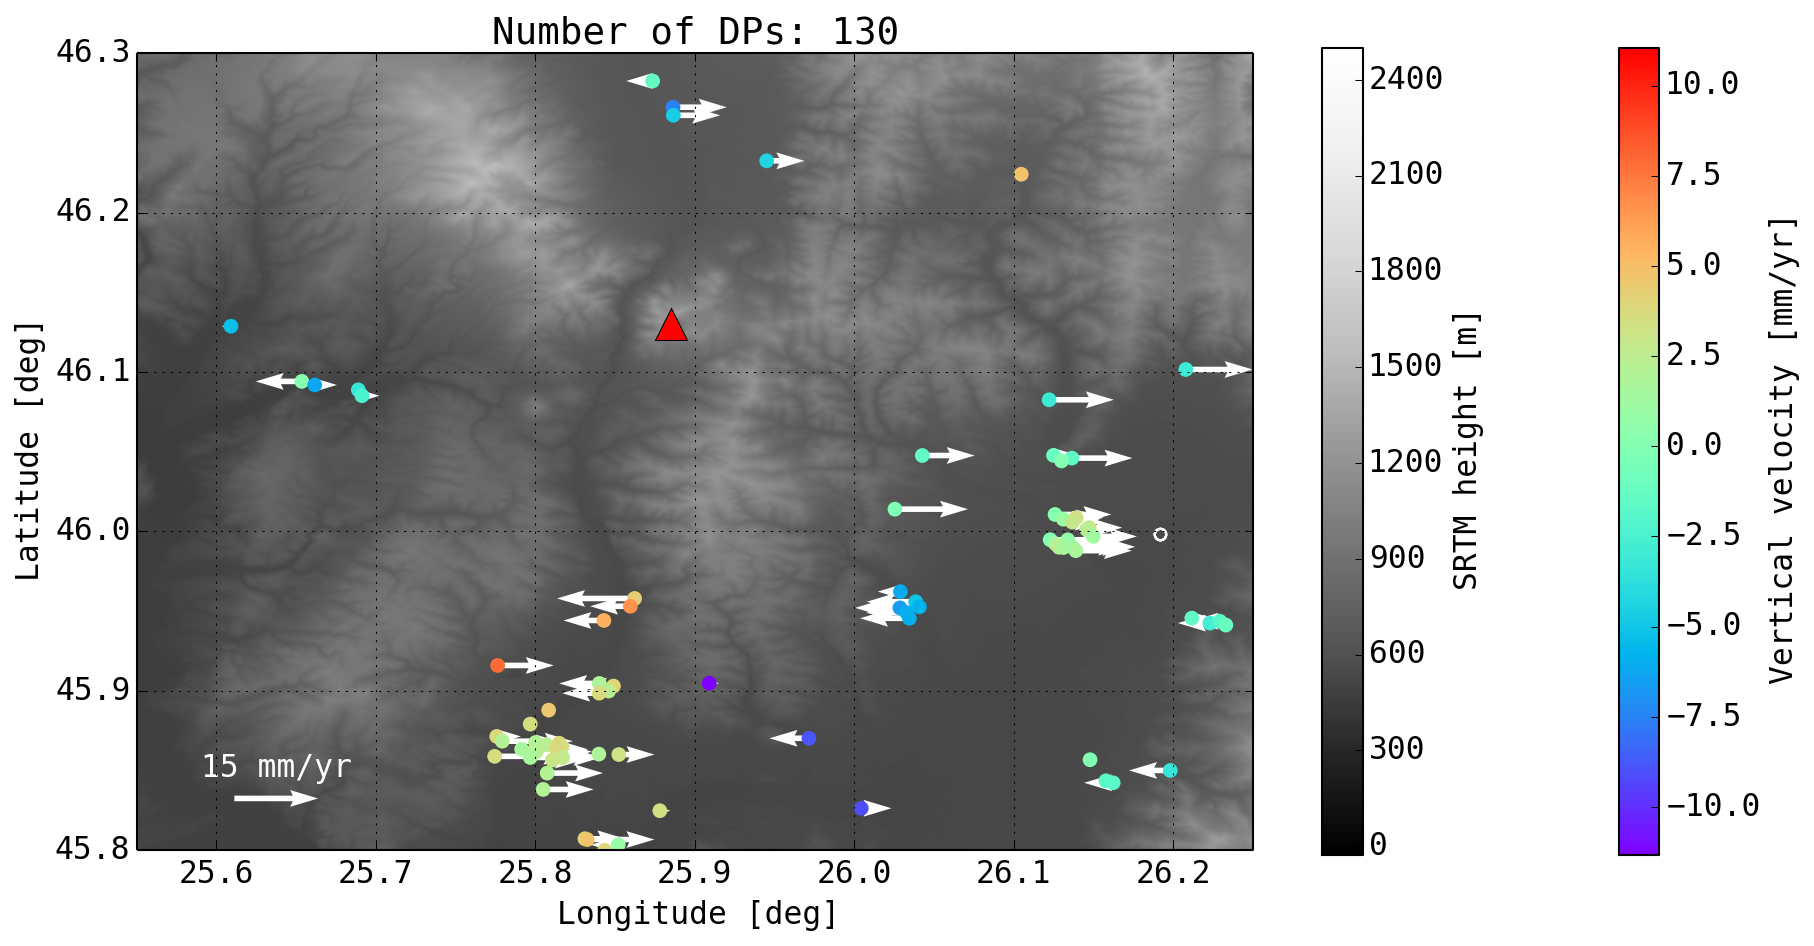
\includegraphics[width=0.8\linewidth]{dp.png}
    \caption{DAISY program által integrált Domináns Pontok térbeli eloszlása. Háttérben az SRTM3 Digitális Magassági Modell \cite{SRTM} látható. A piros háromszög a Csomád-vulkánt jelöli.}\label{dps}
\end{figure}

Mivel a DP-ok eloszlása térben igen inhomogén, a jobb értelmezhetőség érdekében, szabályos rácsra, a rácspontokhoz közeli deformáció értékek felhasználásával, interpoláltam a vertikális (U) és kelet-nyugati sebességkomponenseket. Az interpolált adatpontokat a \ref{dp_vel}. ábrán láthatóak.

\begin{figure}[H]
    \centering
    \includegraphics[width=0.8\linewidth]{grid_dp_vel.png}
    \caption{Szabályos rácsra interpolált vertikális és kelet-nyugati sebességkomponensek. Háttérben az SRTM3 Digitális Magassági Modell \cite{SRTM} látható.}\label{dp_vel}
\end{figure}

A vertikális sebességkomponensek ($\pm 2 \text{mm}/\text{év}$) értéke általában kisebb, mint a kelet-nyugatiaké (jellemzően $\pm 5 \text{mm}/\text{év}$), azaz a mozgás jellemzően a horizontális síkban zajlik. A vertikális jórészt emelkedést mutatnak, a ponthalmaz szélén tapasztalunk csak süllyedést. A kelet-nyugati komponenseket a keleti irányú sebességek dominálják, főleg a É \ang{46.0} és É \ang{46.1} szélességek között. Ahogyan a \ref{GNSS} fejezetben említettem a GNSS mérések \cite{Hoeven2005, Schmitt2007} által meghatározott horizontális sebességek főleg déli enyhén keleti irányú mozgást mutatnak. A GNSS sebességek nagysága nem haladta meg az $1.5 \text{mm}/\text{év}$-et. A műholdradar interferometria, a rendelkezésre álló felvételek felhasználásával az észak-déli sebességkomponensre ugyan érzéketlen, viszont a sebességek nagysága között van némi eltérés (GNSS: $\pm 1.5 \text{mm}/\text{év}$, InSAR: $\pm 5 \text{mm}/\text{év}$).

A \ref{GNSS_vs_insar}. ábrán van der Hoeven és társai \cite{Hoeven2005} által számított és az egyenletes rácsra interpolált InSAR vertikális sebességek láthatóak. A sebességek nagyságrendje és iránya sincs összhangban, bár néhol hasonlóságok felfedezhetőek.

\begin{figure}[H]
    \centering
    \includegraphics[width=\linewidth]{hoeven_gps_vs_insar_vert_colorbar.png}
    \caption{Bal oldali ábrán a \cite{Hoeven2005} által kiszámítitt és interpolált GNSS vertikális sebességek. Jobb oldalt a szabályos rácsra interpolált InSAR vertikális sebességek a \texttt{matplotlib} \cite{matplotlib} \texttt{tricontourf} függvényével megjelenítve.}\label{GNSS_vs_insar}
\end{figure}

Az eltérések a következő okokra vezethetőek vissza: Magukban a GNSS méréssek sem konzisztensek egymással a teljes vizsgálati területen. A mérések meghatározott kampányokban, különböző állandósítási módon, különböző eszközökkel történtek. Emellett a felhasznált interferogramok nem koherens (zajos) területei csökkentik a meghatározott deformációk pontosságát, ezzel a levezetett sebességek megbízhatóságát. Külön problémát okozott a fáziskicsomagolás lépésénél az, hogy a detektált szórópontok nem egyenletesen fedték le a területet, ezzel bizonytalanná vált az egész fázisok (ciklustöbbértelműség) meghatározása. A Csomád-vulkán környékén a felszíni deformációs sebességek kicsik, az interferogramok fázisértékeit nem a deformáció hanem, az egyéb fázistagok (atmoszferikus, DEM- és pályahiba, zaj) dominálták, mely tovább nehezítette a fáziskicsomagolást.

Ezen tényezők hibás fáziskicsomagoláshoz és bizonytalan LOS sebességekhez vezettek.

\chapter{Összefoglalás, eredmények értékelése és kitekintés}

A szakdolgozatom elkészítése során megismerkedtem az InSAR módszer alapfogalmaival és alapelveivel, továbbá alkalmaztam a Csomád-vulkán környékére. Ezen a területen kizárólag GNSS mérésekből származtatott felszíni deformációs sebességek \cite{Hoeven2005, Schmitt2007} álltak rendelkezésre a tudományos közösség számára. A GNSS deformációs sebességek több területen is ellentmondó eredményeket adtak. A műholdradar interferometria egy független ellenőrzési módszert adhat a bekövetkezett deformációk meghatározására.

Dolgozatomban bemutattam a rendelkezésre álló archív Envisat felvételek alapján a \stamps idősorelemzéssel elért eredményeket és összevetettem őket a GNSS  mérések eredményeivel. Annak ellenére, hogy a Csomád vulkán területén nem sikerült megfelelő természetes szórópontokat azonosítani, érdekes megfigyelni, hogy a vulkán tágabb környezetében detektált mozgások koherens keleti irányt mutatnak, amelyek nagysága a Vrancea zóna felé haladva fokozatosan csökken, ezzel együtt a terület keleti részén kismértékű süllyedések figyelhetők meg.
Ez összhangban van van der Hoeven és társainak \cite{Hoeven2005} eredményeivel. A műholdradar interferometriával meghatározott sebességtér értelmezésénél azonban figyelembe kell venni a módszer korlátjait, ezzel együtt a meghatározott sebességek pontosságát.

A területen jelentkező deformációk olyan kis amplitúdójúak, hogy azokat a GNSS mérésekkel is nehéz volt detektálni. A meghatározott interferogramok fázis értékeit nem a deformációs fázis dominálja, hanem más fázistagok (légkör, DEM, zajok, pálya). Ezek megbízható meghatározása az alkalmazott MTInSAR módszerrel elvégezhető feltételezve, hogy megfelelő minőségű interferogramok állnak rendelkezésre. A rendelkezésre álló SAR felvételek időben nem biztosítottak megfelelő lefedettséget, ezért a növényzettel borított területeken nem volt megfelelő koherencia.\\[25pt]
A 2014-ben és 2016-ban az ESA által felbocsájtott műholdak (Sentinel-1A és B) kiküszöbölik a korábbi missziók hiányosságait és közel a teljes földfelszín szisztematikus megfigyelését biztosítják. A Sentinel felvételek közötti időbeli (6-12 nap) és térbeli ($\approx \SI{150}{\meter}$) bázisvonalak sokkal kisebbek mint az általam használt Envisat műhold felvételek esetén. Ezen kisebb bázisvonalak a dolgozatban bemutatott dekorreláció által okozott hibákat és inkoherenciát jelentősen csökkenteni fogják. A felszíni deformációk idősorelemzéséhez több éves felvételsorozat szükséges, mivel a Csomád-vulkán környezetében zajló felszíni deformációk igen lassan mennek végbe, viszont a Sentinel műholdak csak a közelmúltban kezdték meg működésüket.

Emellett a végzett vizsgálatok rámutattak arra, hogy a tektonikai folyamatok által okozott deformációk teljeskörű, 3D-s meghatározása olyan mesterséges szórópontok alapján lehetséges, amely együttesen alkalmasak GNSS mérésekre és interferometrikus adatok feldolgozására. Mesterséges szórópontok (sarokreflektorok) telepítése, a Csomád-vulkán környékére, a vulkán felszíni deformációinak megfigyelésére, már előkészületben van.

\chapter*{Köszönetnyilvánítás}

Szeretnék köszönetet mondani Szűcs Eszternek és Bányai Lászlónak GGI-tól a rengeteg segítségért és jó tanácsért, amit tőlük kaptam, útmutatásuk nagyban hozzájárult szakmai fejlődésemhez.
Köszönet illeti Wesztergom Viktort a GGI Igazgatóját, aki lehetővé tette azt, hogy én is részt vegyek a GGI InSAR projektben.\\[25pt]
Köszönetemet fejezem ki Molnár Gábornak, aki belső konzulensként elvállalta a témát és segített a szakdolgozat elkészítésében.

\newpage

\chapter*{Függelék}

A felhasznált programcsomagok honlapjai:\\
\texttt{ROI\_PAC}: \url{http://www.openchannelfoundation.org/projects/ROI_PAC}\\
\texttt{DORIS}: \url{http://doris.tudelft.nl/}\\
\stamps: \url{https://homepages.see.leeds.ac.uk/~earahoo/stamps/}\\
\texttt{SNAPHU}: \url{https://web.stanford.edu/group/radar/ softwareandlinks/sw/snaphu/}\\
\texttt{DAISY}: \url{http://ggki.hu/~banyai/DAISY/}\\[25pt]
Az ábrák elkészítéséhez a felsorolt feldolgozóprogramokat és a \texttt{python} programnyelvhez készült tudományos programcsomagokat használtam. A felhasznált python könyvtárak:\\
\texttt{matplotlib}: \url{http://matplotlib.org/} \cite{matplotlib}\\
\texttt{numpy}: \url{http://www.numpy.org/} \cite{numpy}\\
\texttt{scipy}: \url{https://www.scipy.org/} \cite{scipy}

\listoftables
\listoffigures

\bibliographystyle{apalike}
\bibliography{../insar}

\newpage

\begin{center}
    {\LARGE \bf{NYILATKOZAT}}
\end{center}
\vspace{10mm}
{\bf Név:} Bozsó István\\
{\bf ELTE Természettudományi Kar, szak:} Geofizika MSc., űrkutató és
távérzékelő szakirány\\
{\bf NEPTUN azonosító:} J9HJKX\\
{\bf Szakdolgozat címe:} Felszíni deformációs sebességek becslése a Csomád vulkán térségében állandó szórópontú radarinterferometria segítségével
\newline{\quad}
\newline{\quad}
\newline{\quad}A {\bf szakdolgozat} szerzőjeként fegyelmi felelősségem tudatában kijelentem, hogy a dolgozatom önálló munkám eredménye, saját szellemi termékem, abban a hivatkozások és idézések standard szabályait következetesen alkalmaztam, mások által írt részeket a megfelelő idézés nélkül nem használtam fel.
\newline{\quad}
\newline{\quad}
\newline{\quad}
\newline{\quad}
Budapest, 2017. május 20.
\begin{flushright}
-----------------------------------------\\
\qquad a hallgató aláírása \qquad\qquad\qquad
\end{flushright}

\end{document}
